\section{Tests}
\label{sec:tests}

{\bf In this section we present three kinds of tests: (1) {\em verification tests}--tests with analytic solutions--that allow us to compare the accuracy of our operator-split method with the unsplit method described in \cite{ReynoldsHayesPaschosNorman2009}; {\em validation tests} chosen for their relevance to the target application; and {\em execution speed tests} where we quantify the relative speed of a large, fully-coupled radiation hydrodynamic simulation with a hydrodynamic simulation with a standard optically thin treatment of photoionization and photoheating. }

\subsection{Verification Tests}
\label{subsec:verification}

The radiation, hydrodynamics and chemistry solvers in {\em Enzo} have been
verified in previous work \citep{ReynoldsHayesPaschosNorman2009}, so we
will not focus on the performance of each individual solver here.
However, what is new in this work is our updated coupling strategy
between the radiation transport and chemistry, that unlike the fully
coupled implicit solver in
\cite{NormanEtAl2007,ReynoldsHayesPaschosNorman2009,NormanReynoldsSo2009},
now splits these solvers apart, with coupling instead based on our
adaptive time-stepping strategy.  

To this end, we focus our verification tests in this paper on two
tests with analytical solutions that exercise only the radiation
transport and chemical ionization/recombination components of {\em Enzo}.
These tests were previously described in
\cite{ReynoldsHayesPaschosNorman2009} (sections 4.5 and 4.6); we
summarize them again here.


\subsubsection{Isothermal ionization of a static neutral hydrogen region}
\label{subsec:test1}

This verification test problem, {\bf matching Test 1 in
\cite{IlievEtAl2006},} focuses on the expansion of an ionized 
hydrogen (HII) region in a uniform gas surrounding a radiation
source.  The problem is simplified through assumption of a static gas
field, and a fixed temperature.  Under these assumptions, the
emitted radiation should rapidly ionize the nearby hydrogen, and then
this ionized region should propagate spherically outward until it
reaches a terminal radius at which ionizations balance with
recombinations, called the Str{\" o}mgren radius.  The radius of
this ionization front, $r(t)$, may be analytically computed as
\begin{equation}
  \label{Iliev1_solution}
  r(t) = r_s \left(1-e^{-t/t_{rec}}\right)^{1/3}, \quad\mbox{where}\quad
  r_s = \left(\frac{3\,\dot{N}_{\gamma}}{4\pi\,\alpha_B\,n_H^2}\right)^{1/3}.
\end{equation}
Here, $r_s$ is the Str{\" o}mgren radius, $t_{rec} =
(\alpha_B\,n_H)^{-1}$ is the recombination time, $\dot{N}_{\gamma}$ is
the photon emission rate, $n_H$ is the hydrogen number
density of the gas, and $\alpha_B$ is the case B hydrogen
recombination rate.

In our tests, we use parameters $\dot{N}_{\gamma} = 5\times10^{48}$
photons s$^{-1}$, $n_H = 10^{-3}$ cm$^{-3}$, $\alpha_B =
2.59\times10^{-12}$ cm$^2$s$^{-1}$, domain $[0,6.6\, \mbox{kpc}]^3$,
temperature $T=10^4$ K, and time interval $[0,5\, \mbox{Myr}]$.  The
ionization source is assumed to be monochromatic, at the HI ionization
frequency $h\nu = 13.6$ eV, and is located at the location $(0,0,0)$.
For initial conditions, we use $E = 10^{-45}$ erg cm$^{-3}$ and
ionization fraction HII/H = 0.0012.  We employ reflecting boundary
conditions for the radiation field at the $x=0$, $y=0$, and $z=0$
faces, and outflow boundary conditions at the other three faces.

We plot spherically-averaged radial profiles of the radiation energy
density and the ionization fractions at 10 Myr, 100 Myr and 500 Myr
from a simulation using a 128$^3$ spatial grid and time step
tolerance $\tau_{tol} = 10^{-4}$ in Figure \ref{fig:i1_results},
showing the expected propagation of the radiation front and resulting
I-front in time.
\begin{figure}[t]
\centerline{\hfill
  %% 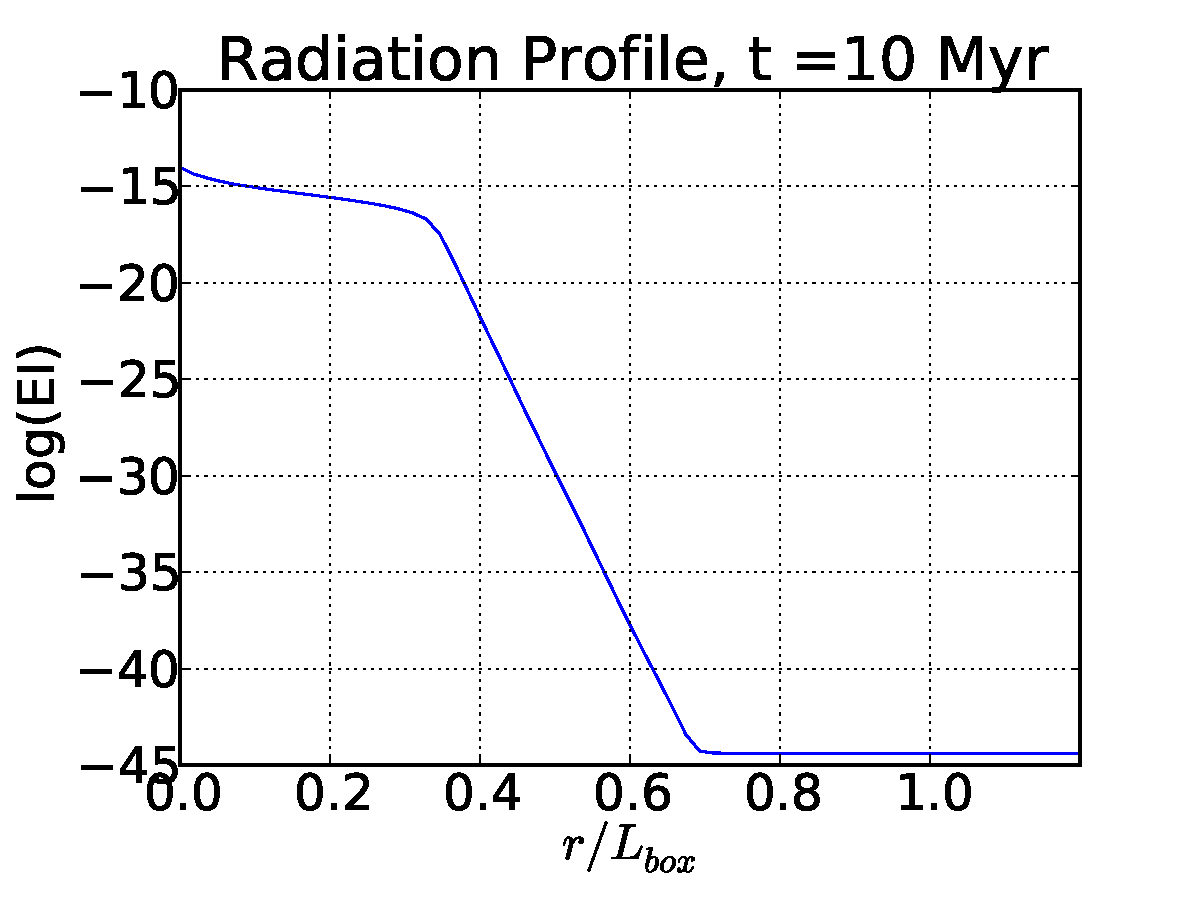
\includegraphics[scale=0.3, trim=1.0cm 0.5cm 1.0cm 0.5cm]{i1-Eprofiles_10Myr.eps}
  %% 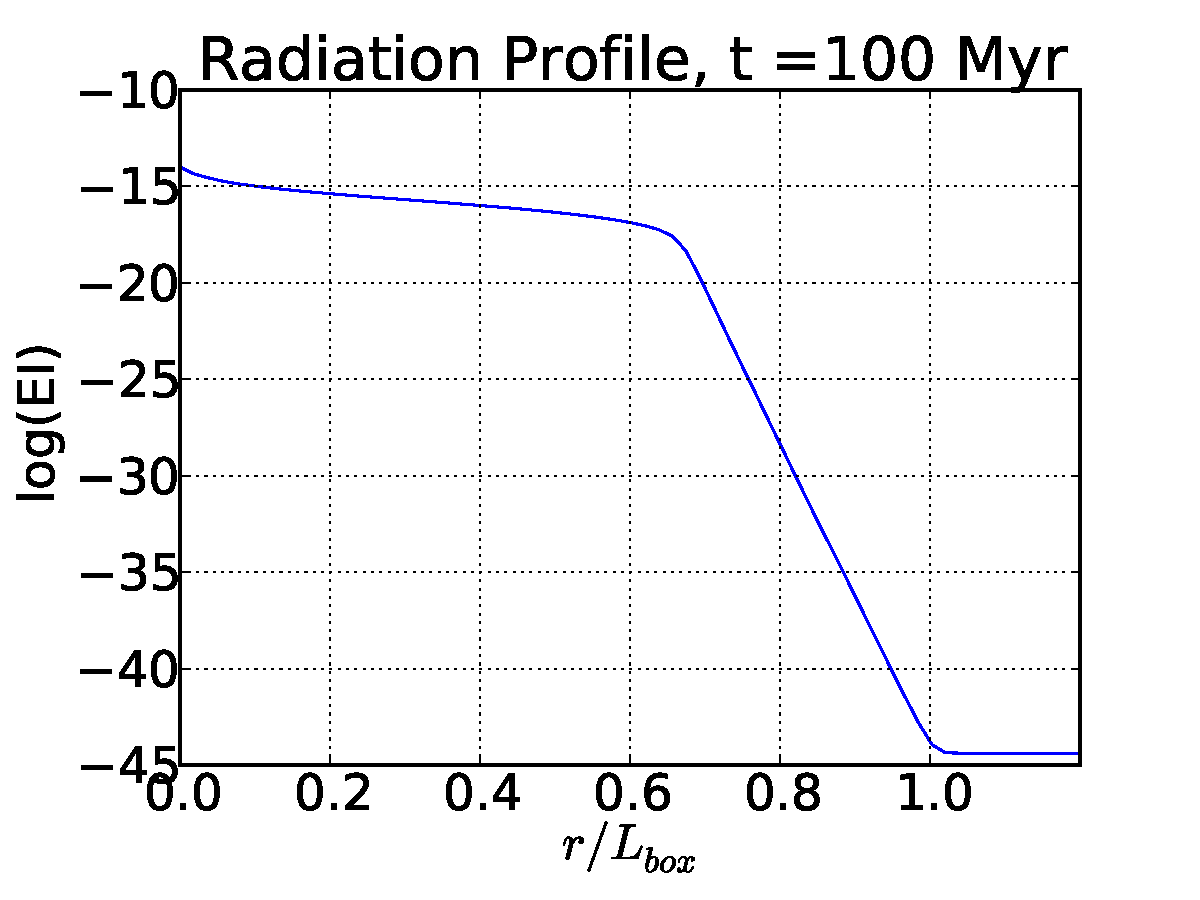
\includegraphics[scale=0.3, trim=1.0cm 0.5cm 1.0cm 0.5cm]{i1-Eprofiles_100Myr.eps}
  %% 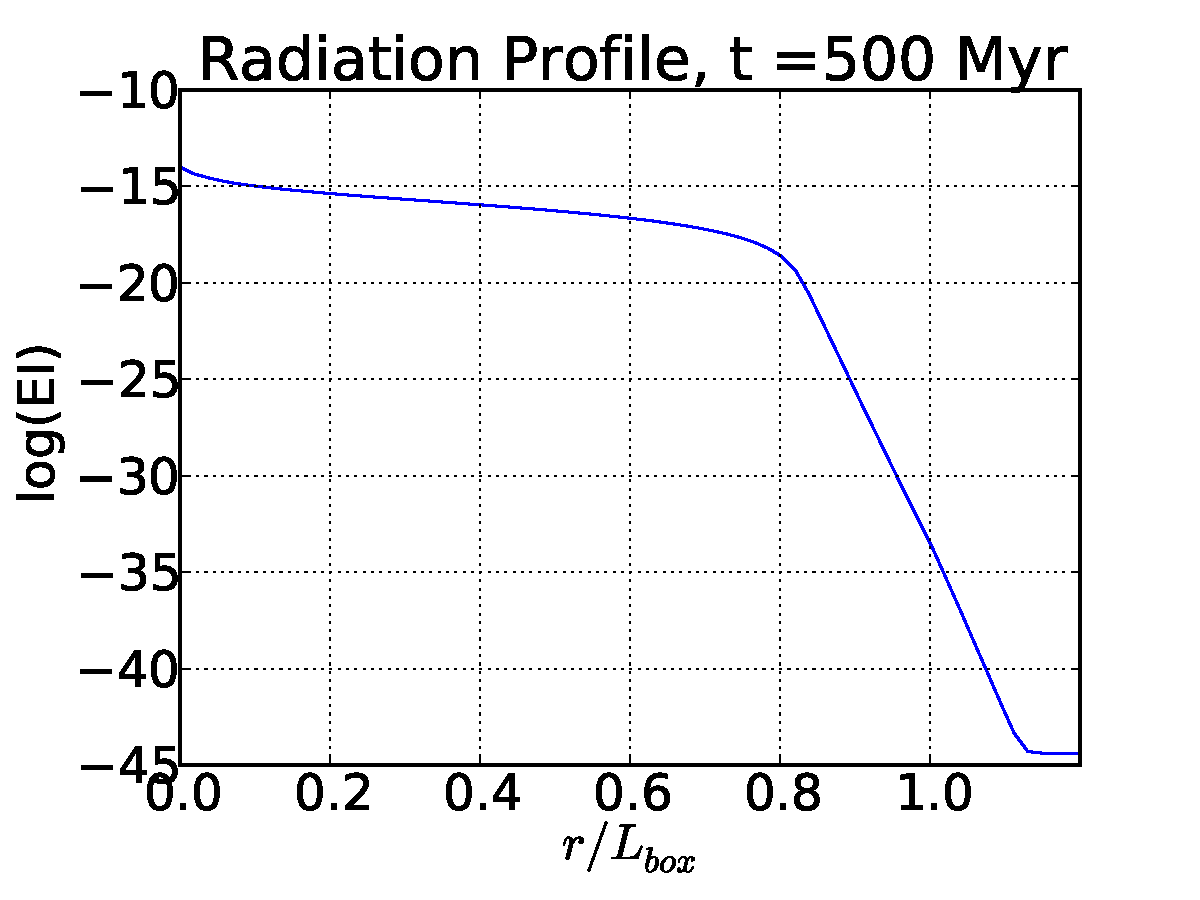
\includegraphics[scale=0.3, trim=1.0cm 0.5cm 1.0cm 0.5cm]{i1-Eprofiles_500Myr.eps}
  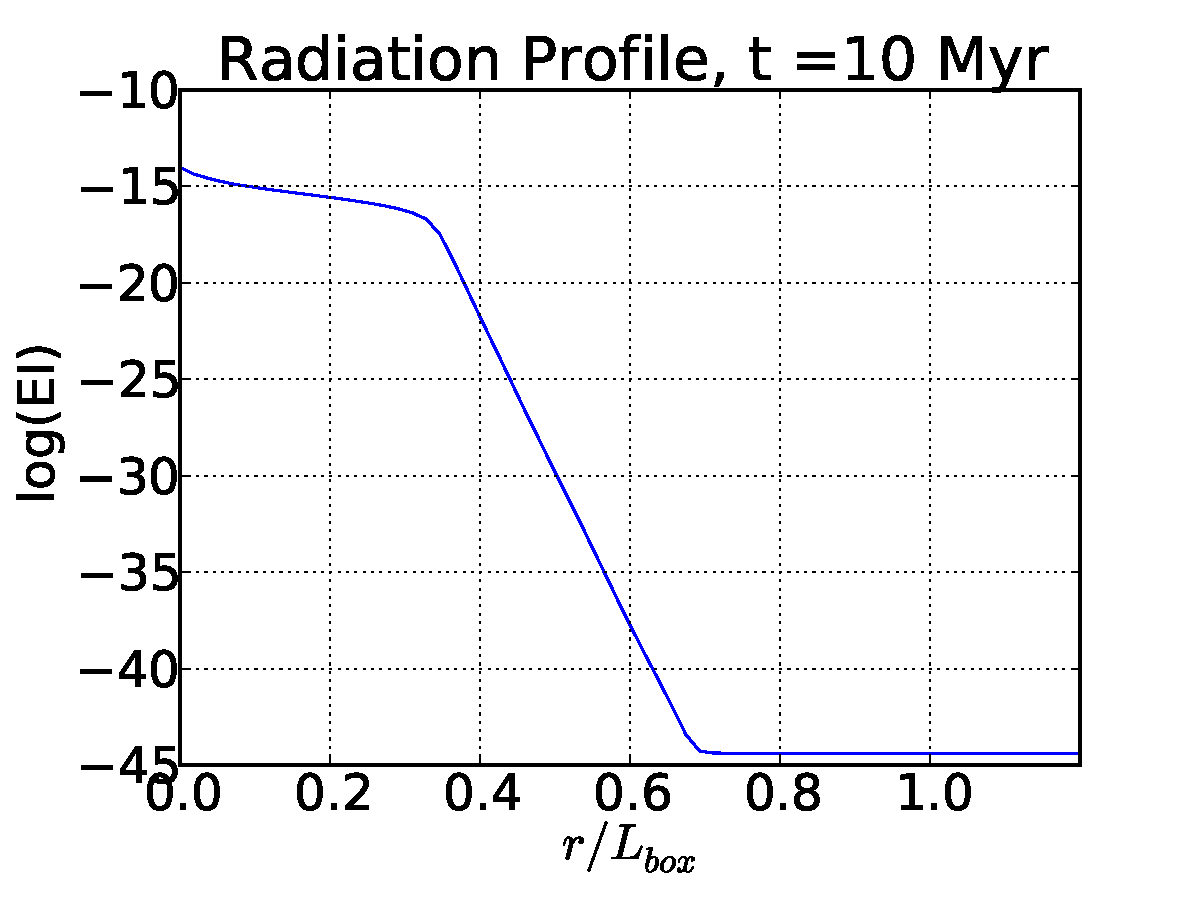
\includegraphics[scale=0.3, trim=1.0cm 1.0cm 1.0cm 0.5cm]{i1-Eprofiles_10Myr.pdf}
  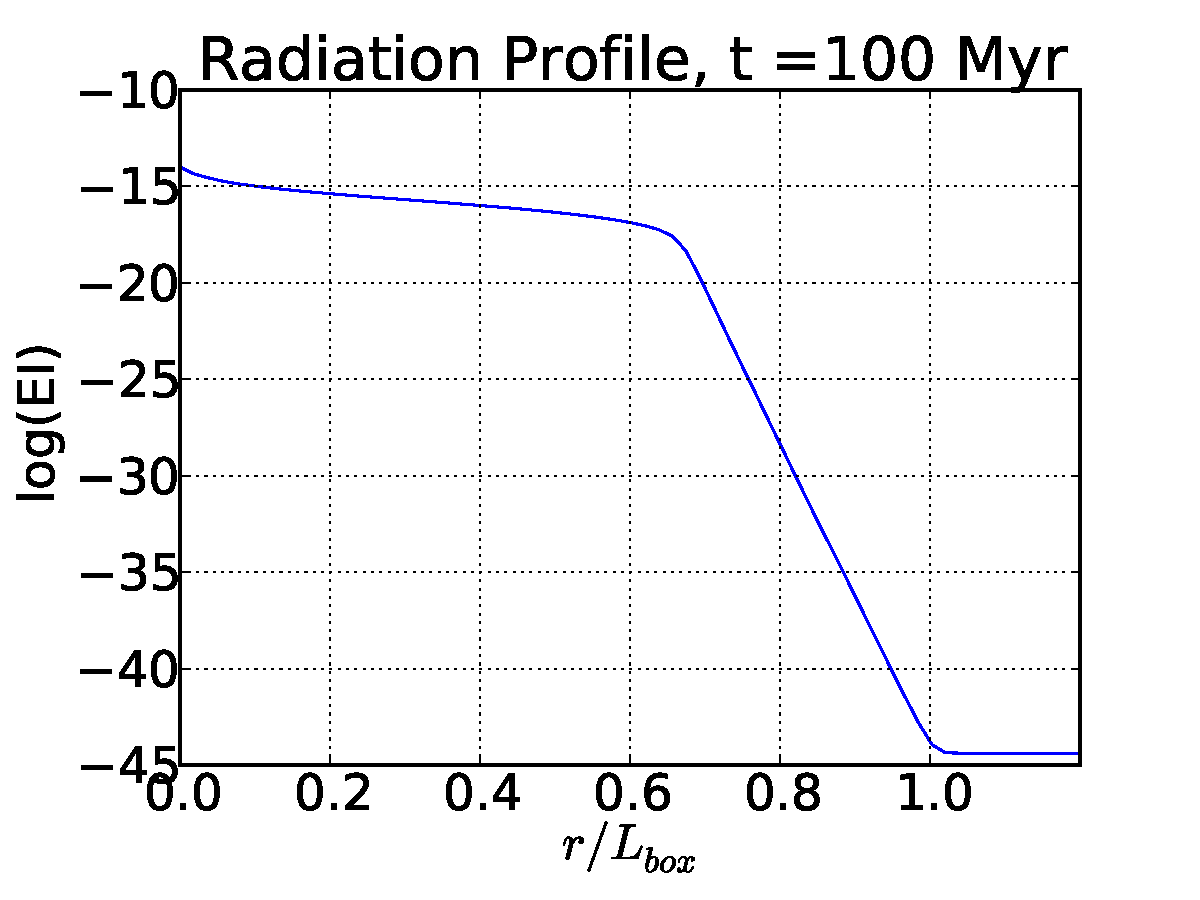
\includegraphics[scale=0.3, trim=1.0cm 1.0cm 1.0cm 0.5cm]{i1-Eprofiles_100Myr.pdf}
  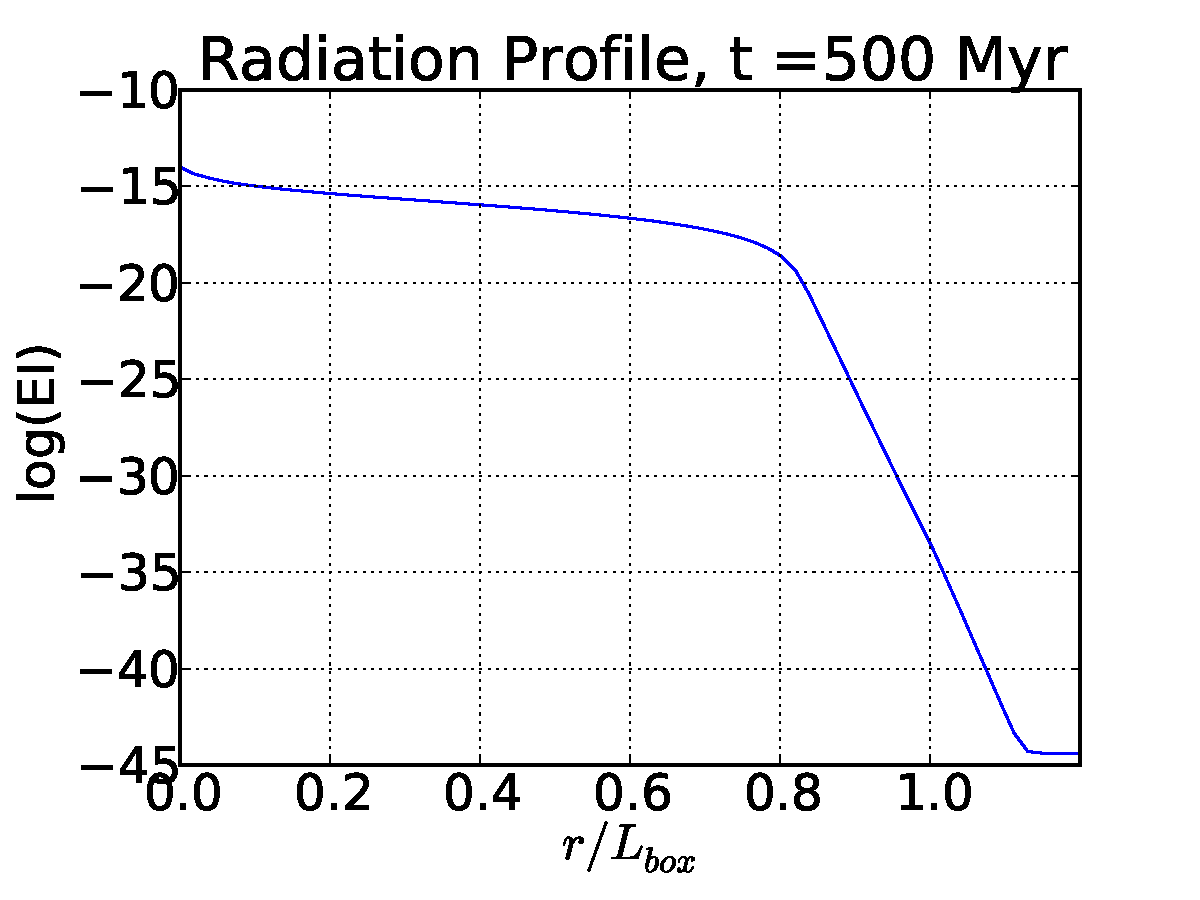
\includegraphics[scale=0.3, trim=1.0cm 1.0cm 1.0cm 0.5cm]{i1-Eprofiles_500Myr.pdf}
  \hfill}
\centerline{\hfill
  %% 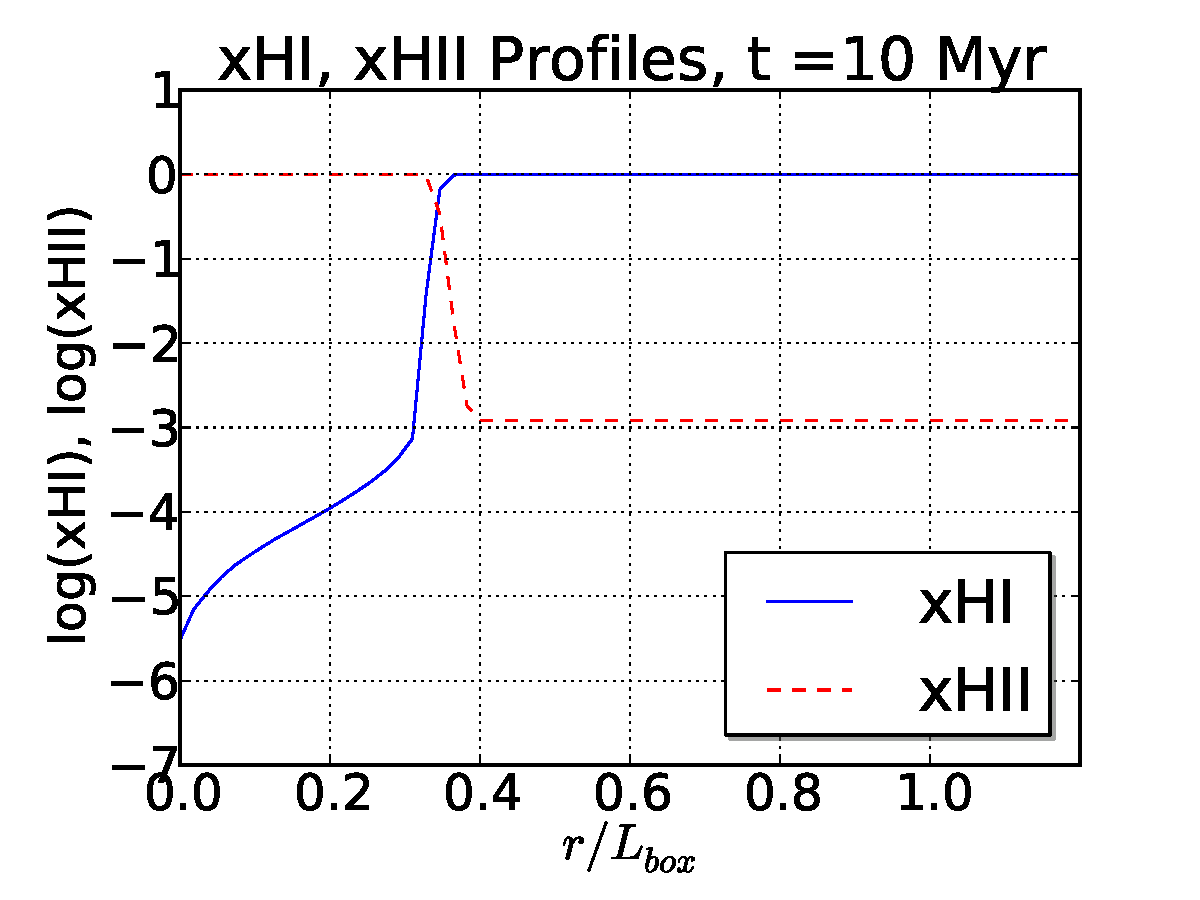
\includegraphics[scale=0.3, trim=1.0cm 0.5cm 1.0cm 0.5cm]{i1-profiles_10Myr.eps}
  %% 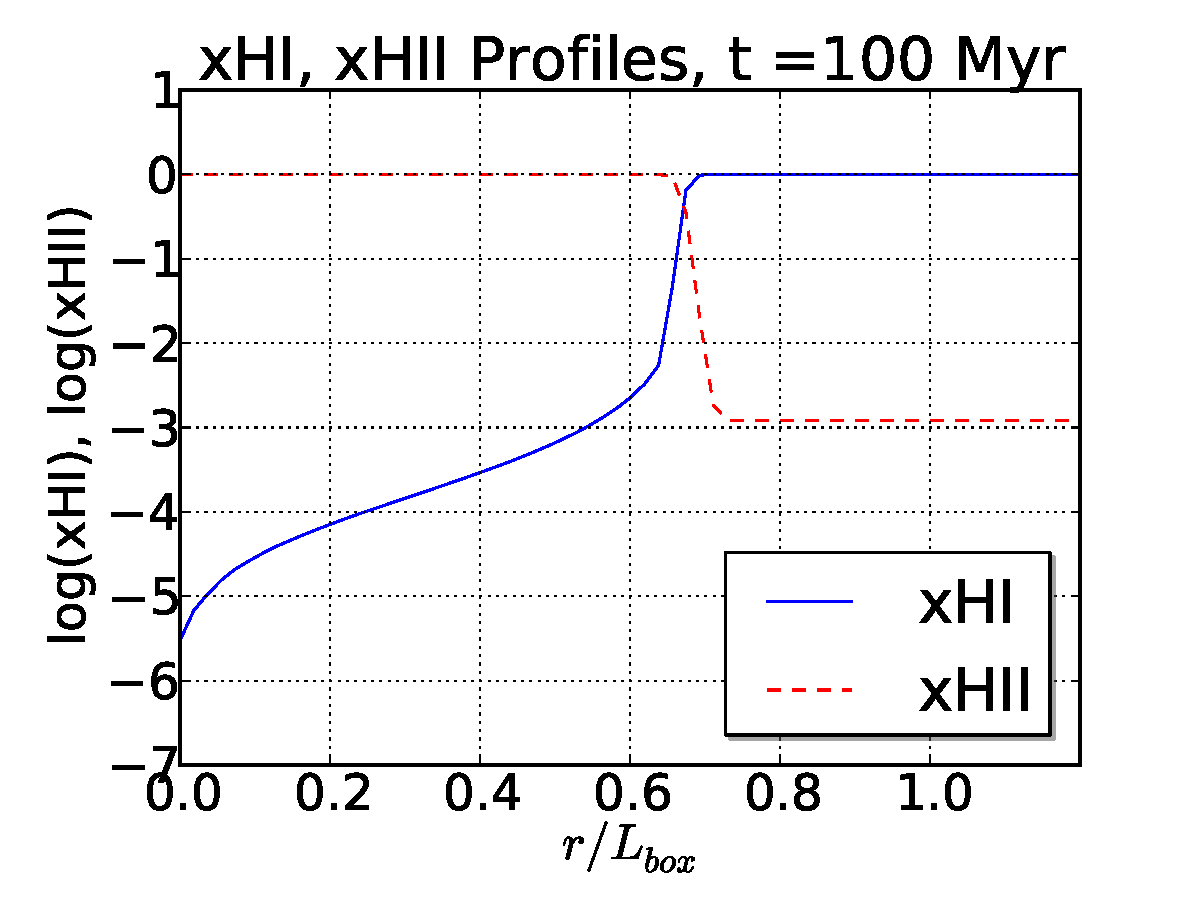
\includegraphics[scale=0.3, trim=1.0cm 0.5cm 1.0cm 0.5cm]{i1-profiles_100Myr.eps}
  %% 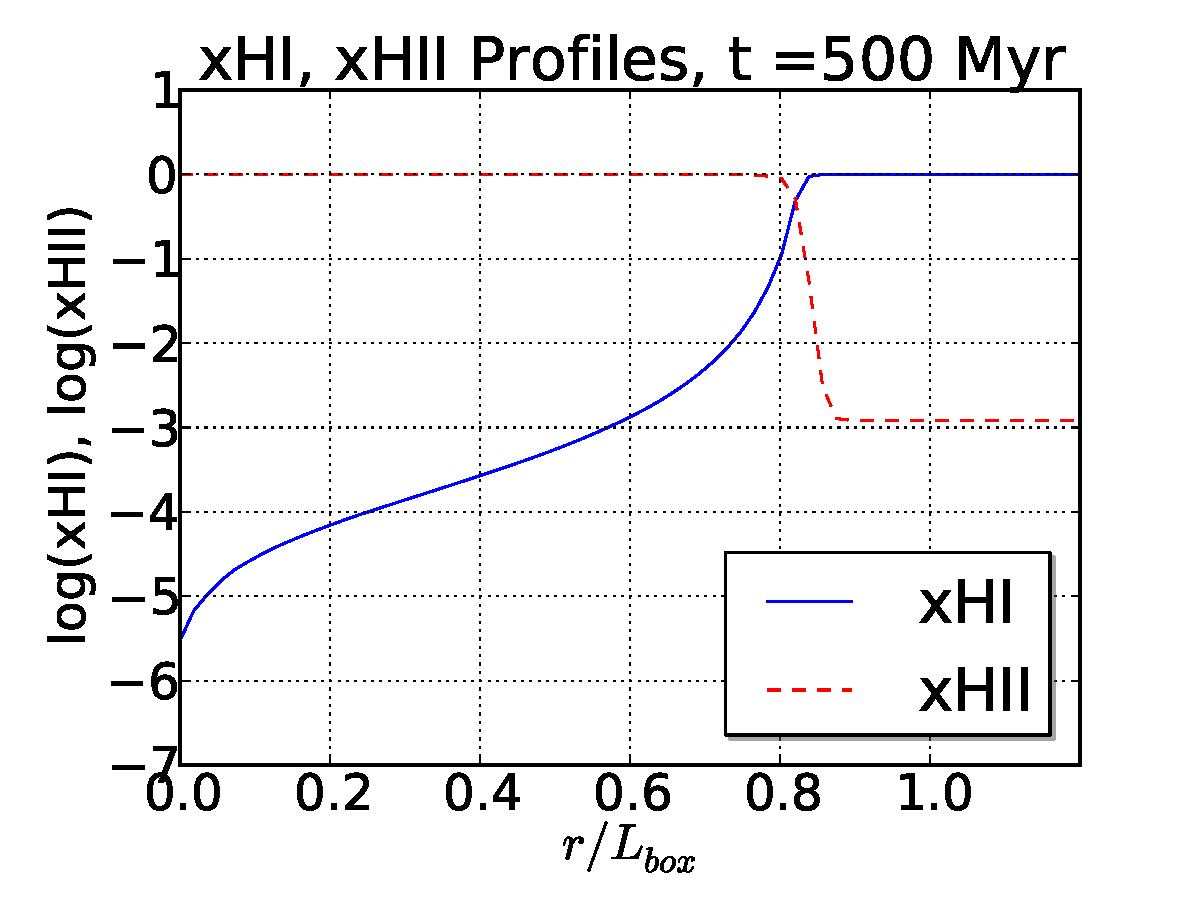
\includegraphics[scale=0.3, trim=1.0cm 0.5cm 1.0cm 0.5cm]{i1-profiles_500Myr.eps}
  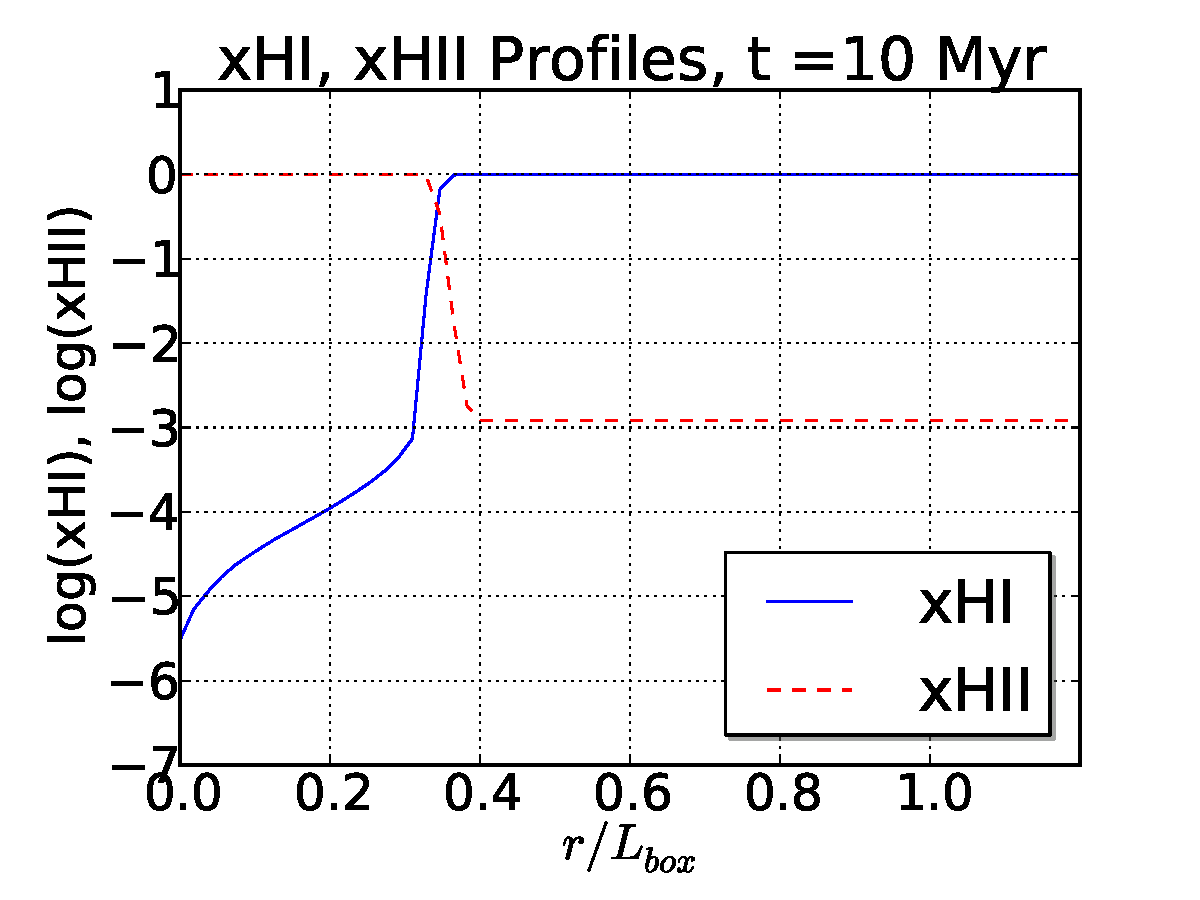
\includegraphics[scale=0.3, trim=1.0cm 0.5cm 1.0cm 0.5cm]{i1-profiles_10Myr.pdf}
  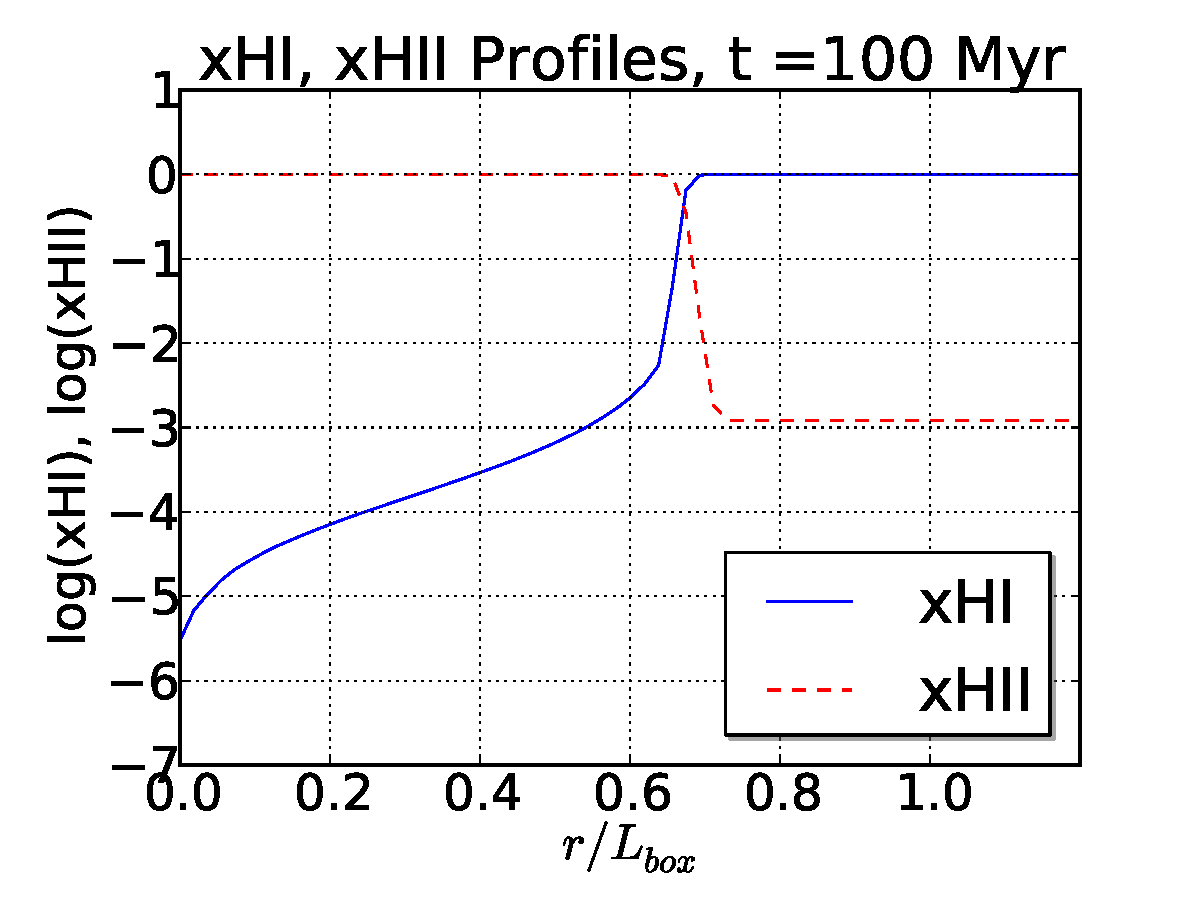
\includegraphics[scale=0.3, trim=1.0cm 0.5cm 1.0cm 0.5cm]{i1-profiles_100Myr.pdf}
  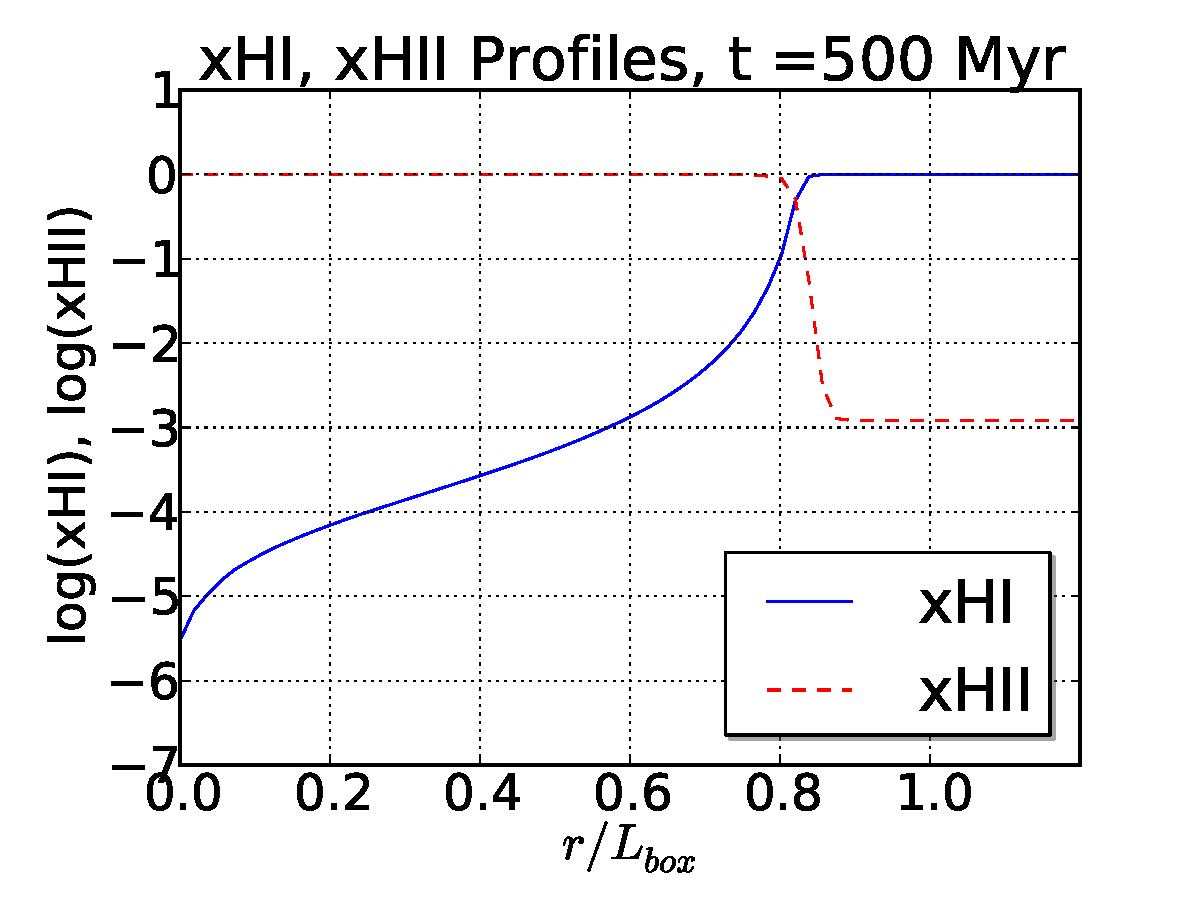
\includegraphics[scale=0.3, trim=1.0cm 0.5cm 1.0cm 0.5cm]{i1-profiles_500Myr.pdf}
  \hfill}
  \caption{Spherically-averaged radial profiles of radiation energy
    density and ionization fractions for the isothermal ionization
    test in section \ref{subsec:test1} using a $128^3$ mesh and
    time step tolerance $\tau_{tol} =10^{-4}$.  Plots are shown at 10, 100
    and 500 Myr (left to right), with the radiation energy density on
    the top row and ionization fractions on the bottom row.}
  \label{fig:i1_results}
\end{figure}
Plots of the computed and analytical I front position and resulting
error for this run are provided in Figure \ref{fig:i1_radius}.
\begin{figure}[t]
\centerline{\hfill
  %% 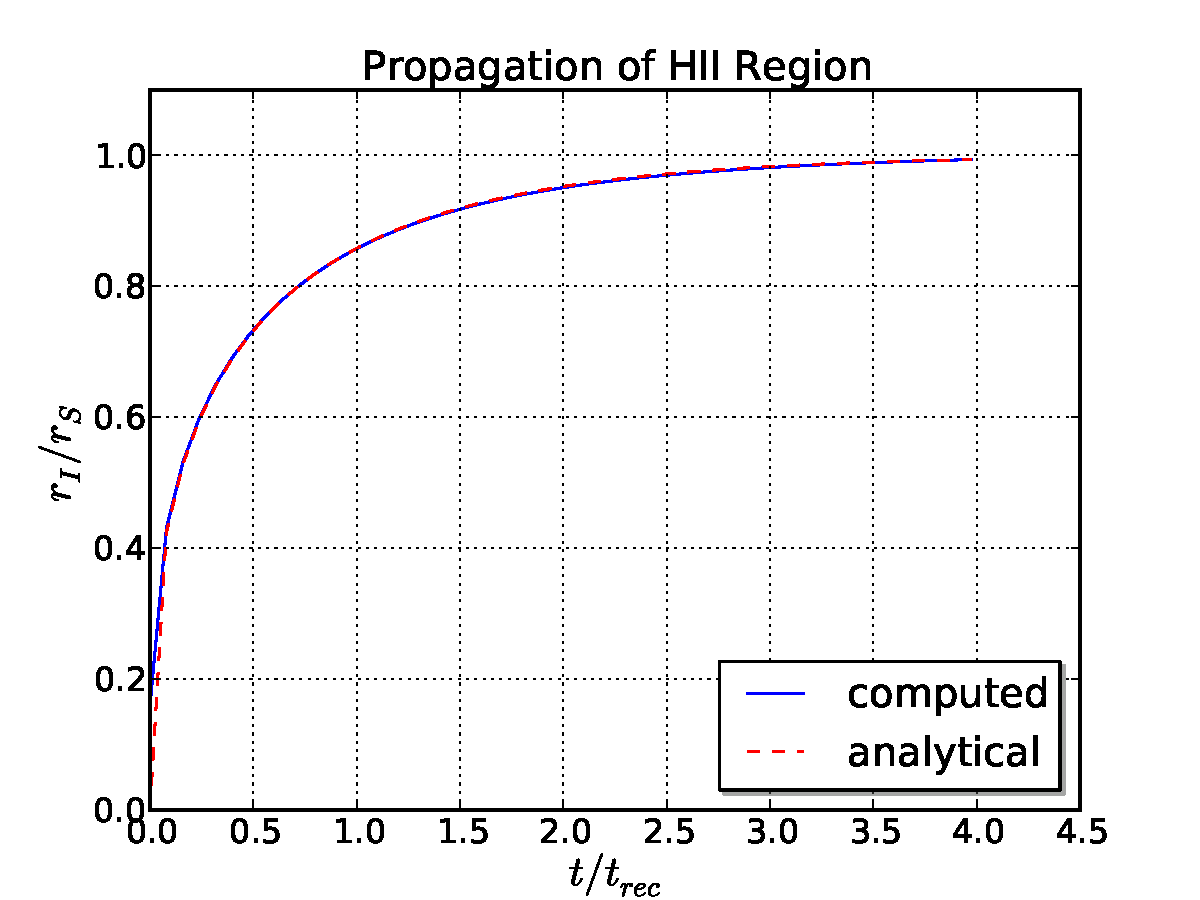
\includegraphics[scale=0.45, trim=1.0cm 0.5cm 1.0cm 0.5cm]{i1-rad_vs_time.eps}
  %% 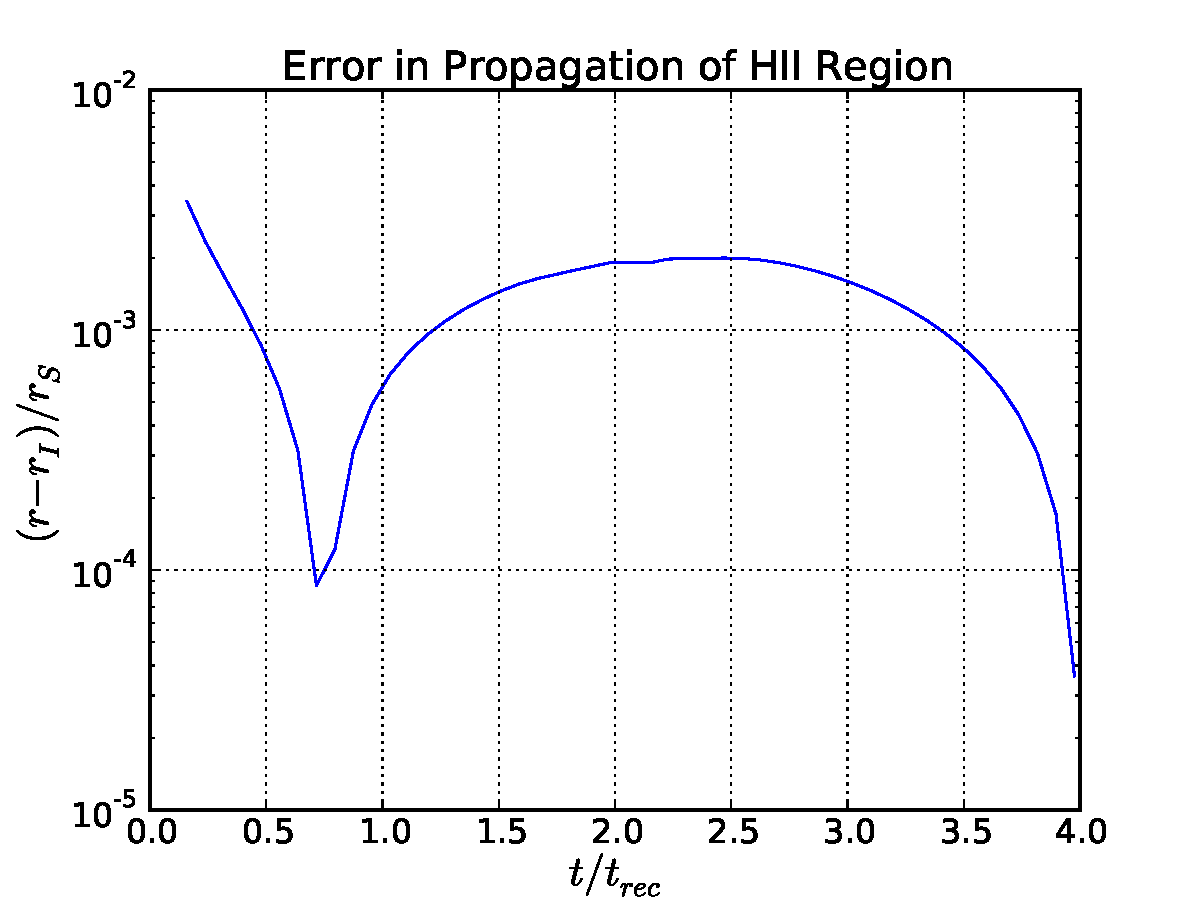
\includegraphics[scale=0.45, trim=1.0cm 0.5cm 1.0cm 0.5cm]{i1-rad_error_vs_time.eps}
  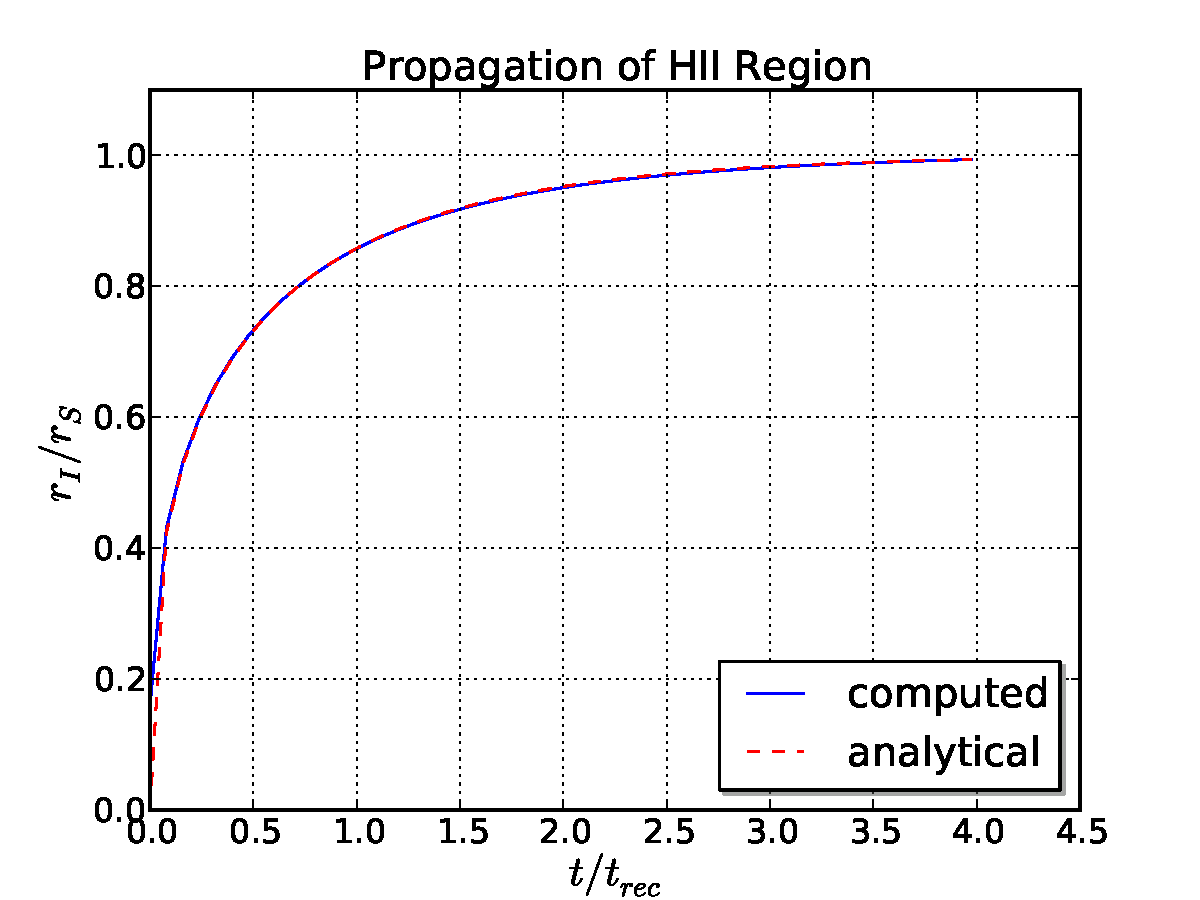
\includegraphics[scale=0.45, trim=1.0cm 0.5cm 1.0cm 0.5cm]{i1-rad_vs_time.pdf}
  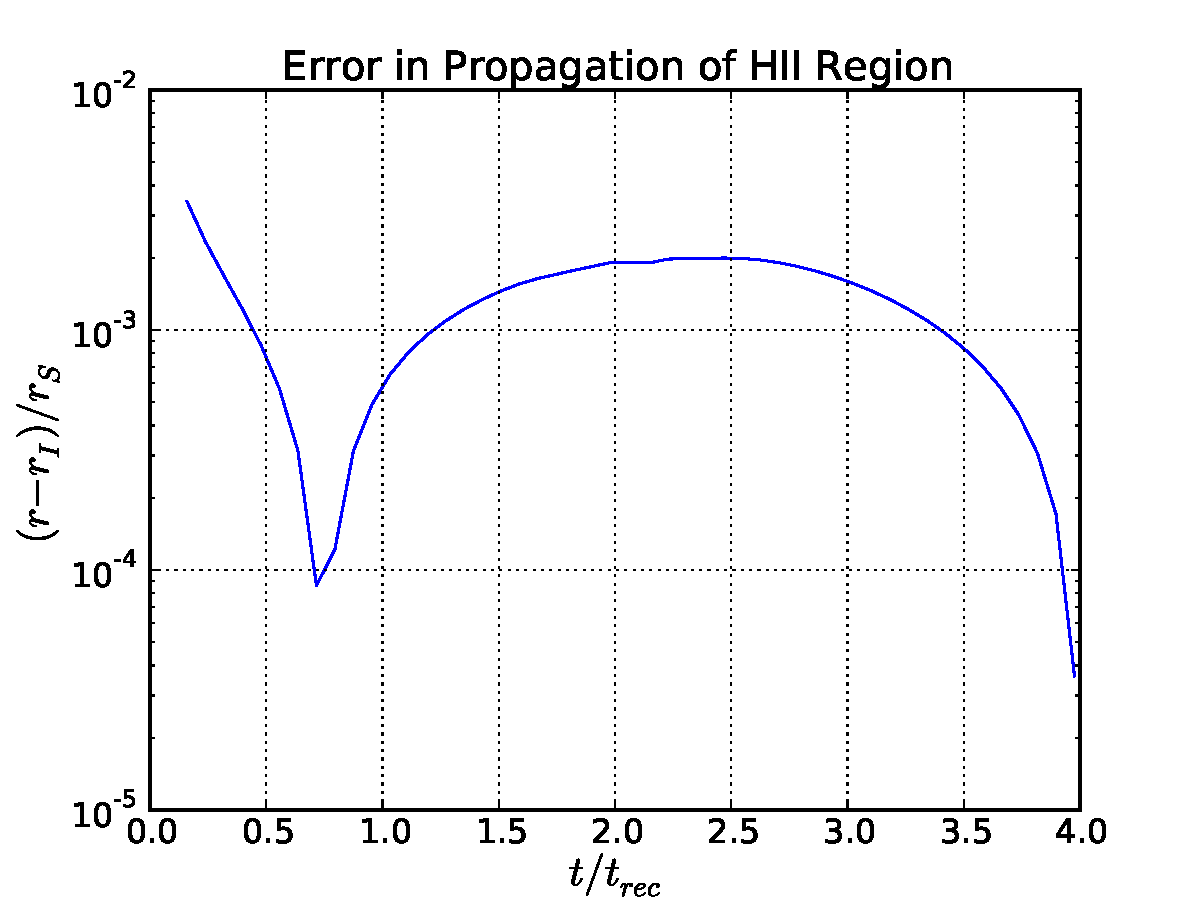
\includegraphics[scale=0.45, trim=1.0cm 0.5cm 1.0cm 0.5cm]{i1-rad_error_vs_time.pdf}
  \hfill}
  \caption{Comparison between computed and analytical I front position
    for the isothermal ionization test in section \ref{subsec:test1}
    using a $128^3$ mesh and time step tolerance $\tau_{tol}
    =10^{-4}$. Solution on left, error on right.} 
  \label{fig:i1_radius}
\end{figure}
To further investigate the accuracy of our new splitting approach
between the radiation and chemistry solvers, we then performed these
same tests at a variety of mesh sizes and time step tolerances 
$\tau_{tol}$.  For mesh sizes of $16^3$, $32^3$ and $64^3$, and for
tolerances $10^{-2}$, $10^{-3}$, $10^{-4}$ and $10^{-5}$, we
compute the error in the I front position as
\begin{equation}
\label{eq:i1_error}
   error \ = \ \left\| \frac{r_{computed} - r_{true}}{r_s} \right\|_{RMS}
   \ = \ \left(\frac{1}{N_t} \sum_{i=1}^{N_t} \left(\frac{r_{computed,i} -
       r_{true,i}}{r_s}\right)^2 \right)^{1/2}.
\end{equation}
In Figure \ref{fig:i1_stats}, we plot the solution error as a function
of the average time step size, as well as the total runtime as a
function of the average time step size.  
\begin{figure}[t]
\centerline{\hfill
  %% 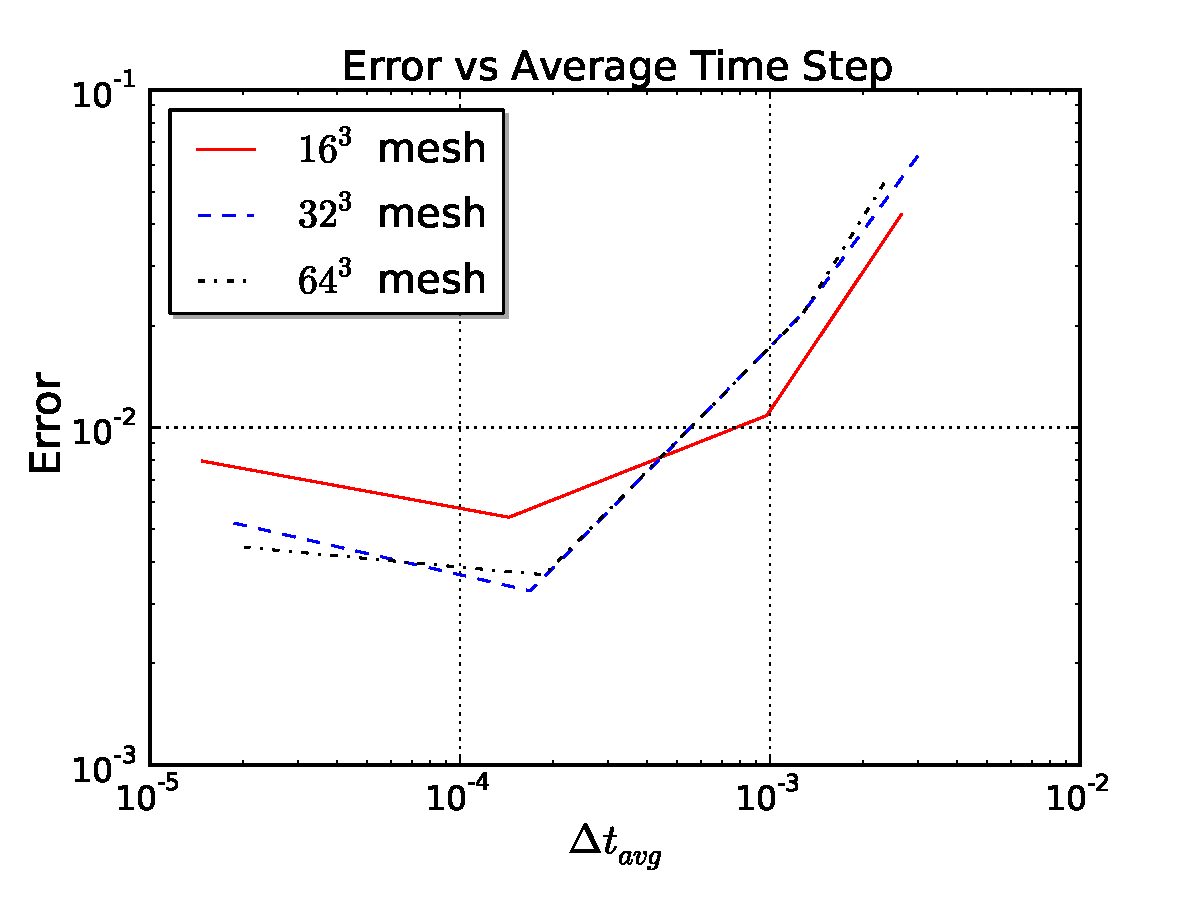
\includegraphics[scale=0.45, trim=1.0cm 0.5cm 1.0cm 0.5cm]{i1-error_enzo.eps}
  %% 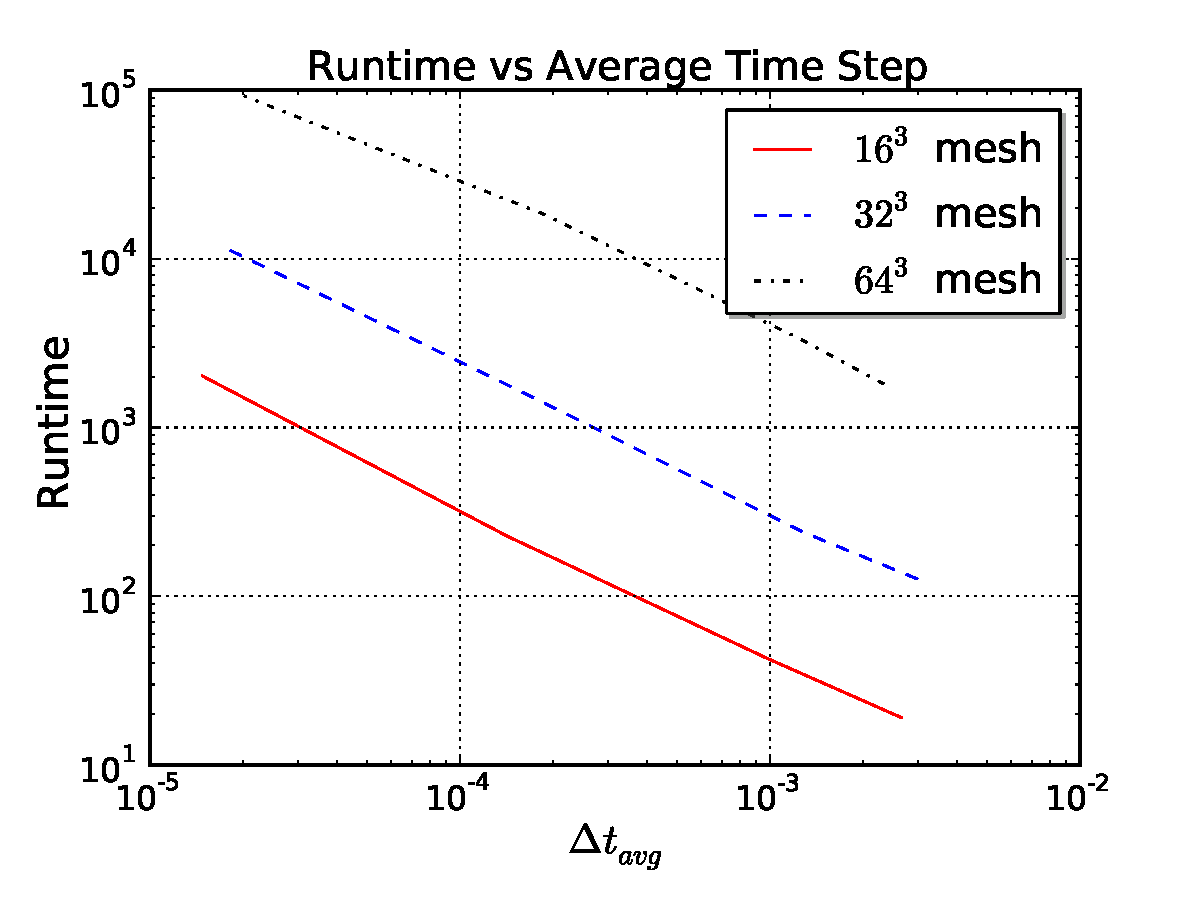
\includegraphics[scale=0.45, trim=1.0cm 0.5cm 1.0cm 0.5cm]{i1-runtime_enzo.eps}
  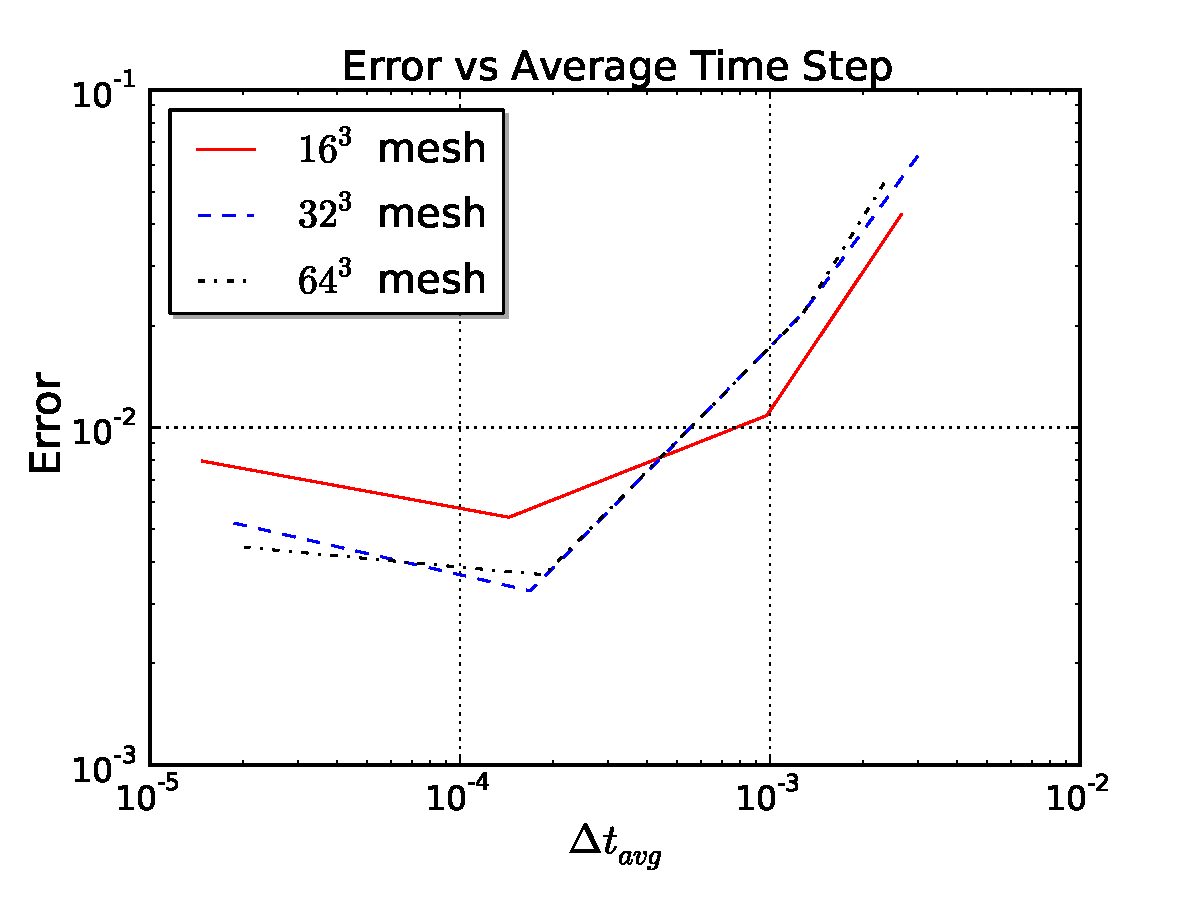
\includegraphics[scale=0.45, trim=1.0cm 0.0cm 1.0cm 0.5cm]{i1-error_enzo.pdf}
  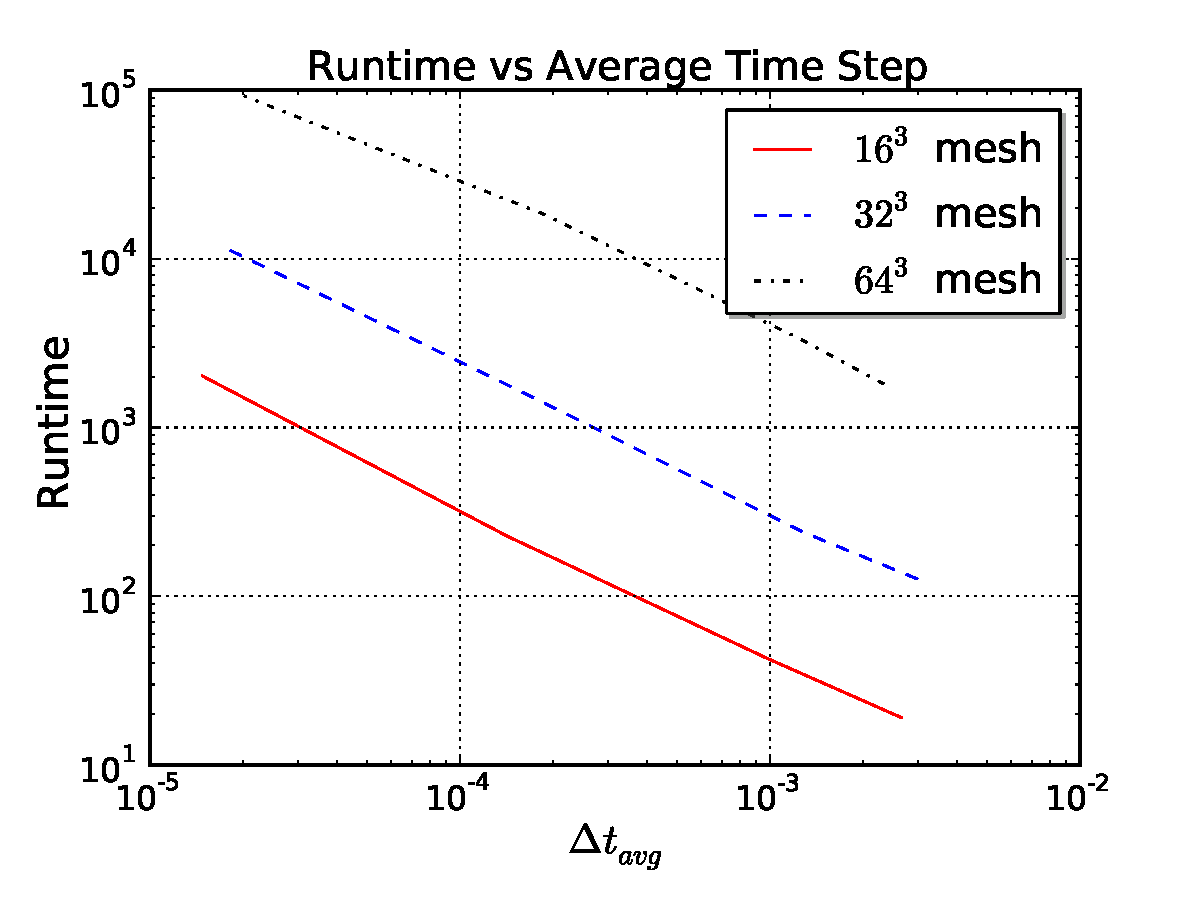
\includegraphics[scale=0.45, trim=1.0cm 0.0cm 1.0cm 0.5cm]{i1-runtime_enzo.pdf}
  \hfill}
  \caption{We ran tests using mesh sizes of
    $16^3$, $32^3$ and $64^4$, and time step tolerances of
    $10^{-2}$, $10^{-3}$, $10^{-4}$ and $10^{-5}$, and plot the I
    front position error \eqref{eq:i1_error} as a function of the
    average time step size.  As expected, the runtime scales linearly
    with the inverse $\Delta t_{avg}$, and the error scales linearly
    with $\Delta t_{avg}$, at least until other sources of error
    dominate the calculation.}
  \label{fig:i1_stats}
\end{figure}
As can be seen in these plots, as the tolerance decreases, the
temporal solution accuracy increases linearly until we reach a minimum
accuracy that results from other components in Enzo (spatial
discretization accuracy, accuracy within Enzo's chemistry solver,
etc.).  Moreover, it is evident that as we decrease the time step
tolerances, the required runtime increases linearly.  These results
imply that there is a ``sweet spot'' in our approach, wherein a
tolerance of $\tau_{tol}=10^{-4}$ achieves the solution with optimal
accuracy before we begin to waste additional effort without achieving
accuracy improvements.  {\bf While this specific value is likely
problem-dependent, we use it as a starting point in subsequent
simulations. }

Finally, in Figure \ref{fig:i1_contours} we plot a slice of the
computed HII region through the center of the domain, perpendicular to
the $z$-direction (other directions are equivalent), to show the
convergence of the ionized region to a sphere at varying spatial
resolutions.
\begin{figure}[t]
\centerline{\hfill
  %% 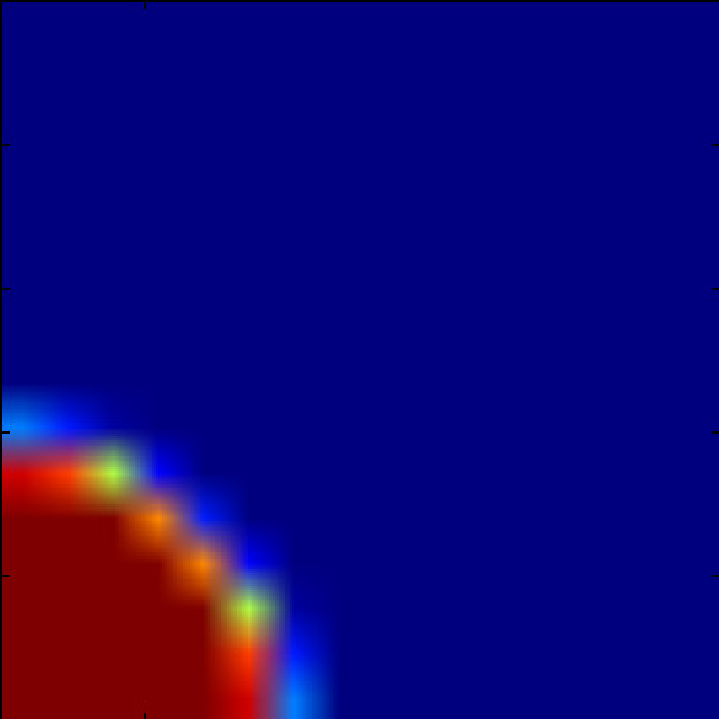
\includegraphics[scale=0.3]{i1-HIIcontour_10myr_nx16.eps}
  %% \hspace{0.1cm}
  %% 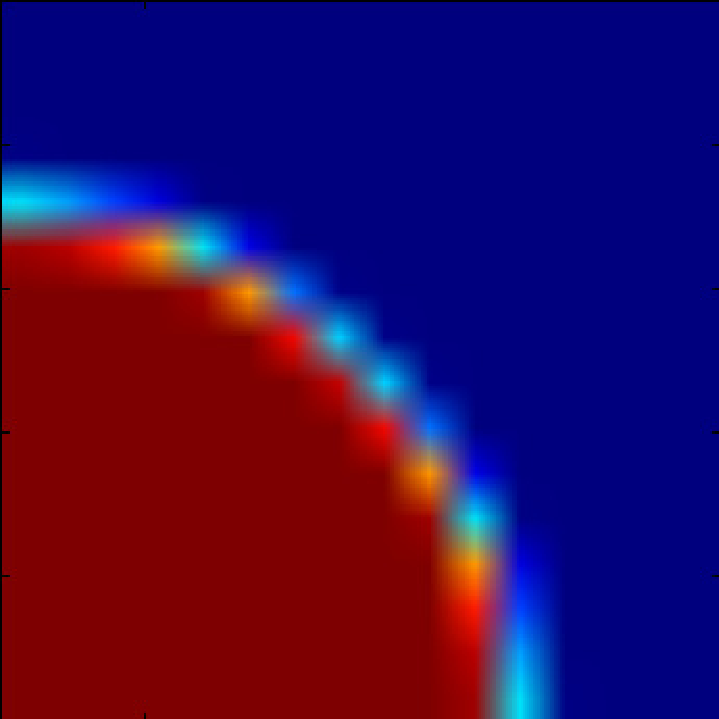
\includegraphics[scale=0.3]{i1-HIIcontour_100myr_nx16.eps}
  %% \hspace{0.1cm}
  %% 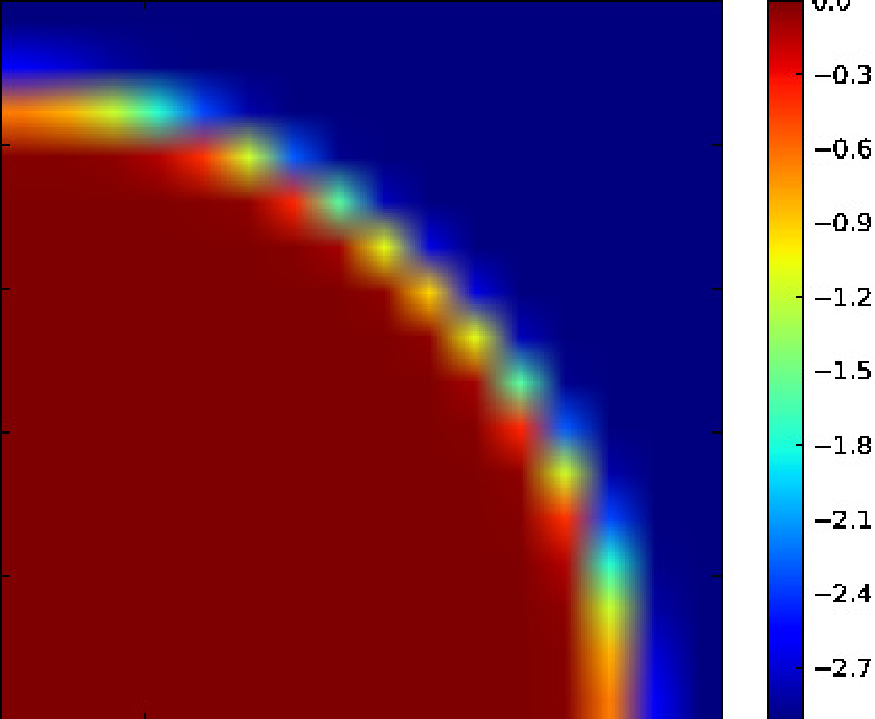
\includegraphics[scale=0.3]{i1-HIIcontour_500myr_nx16.eps}
  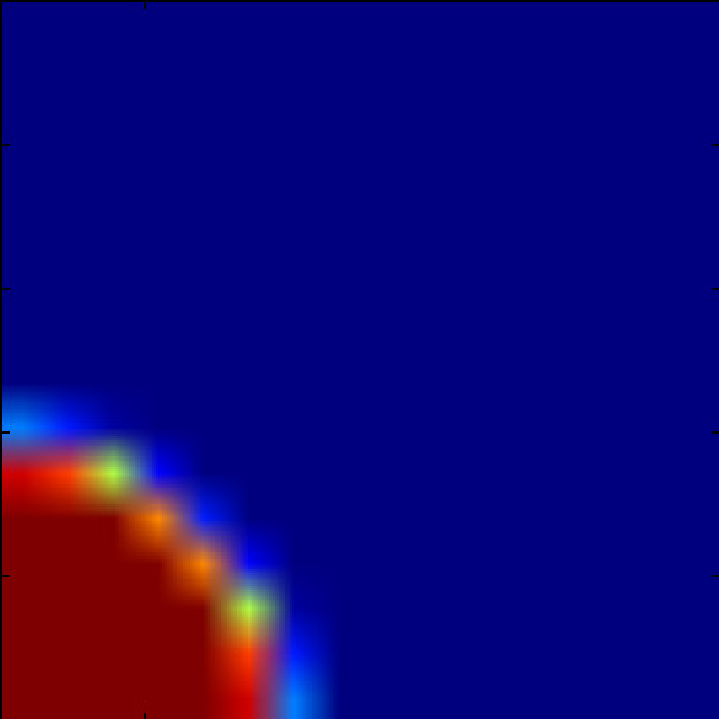
\includegraphics[scale=0.3]{i1-HIIcontour_10myr_nx16.pdf}
  \hspace{0.1cm}
  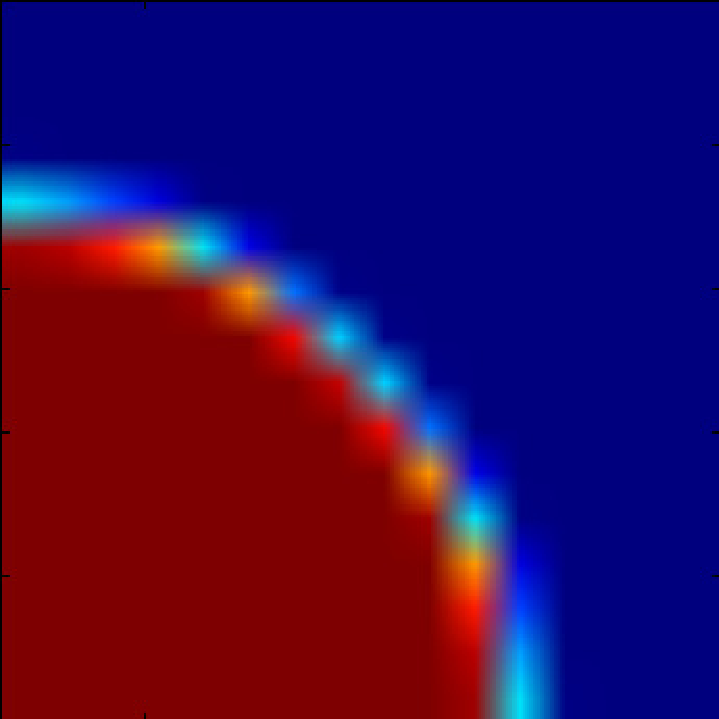
\includegraphics[scale=0.3]{i1-HIIcontour_100myr_nx16.pdf}
  \hspace{0.1cm}
  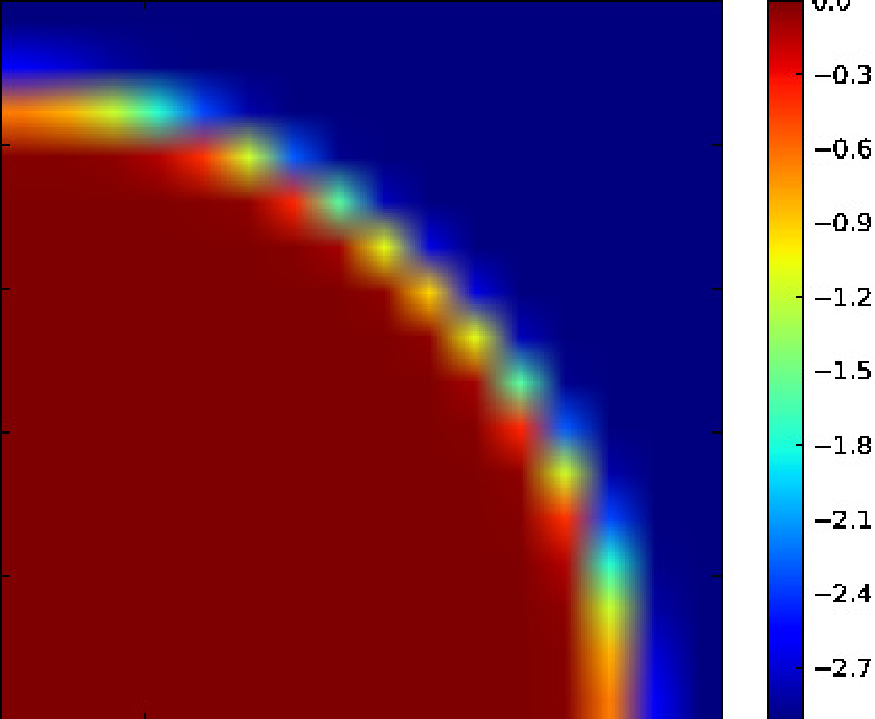
\includegraphics[scale=0.3]{i1-HIIcontour_500myr_nx16.pdf}
  \hfill}
\vspace{0.2cm}
\centerline{\hfill
  %% 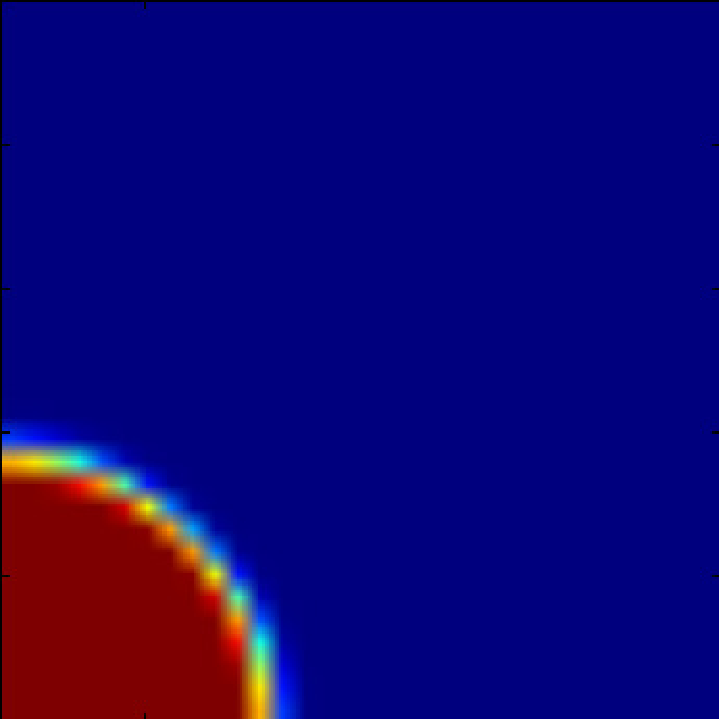
\includegraphics[scale=0.3]{i1-HIIcontour_10myr_nx32.eps}
  %% \hspace{0.1cm}
  %% 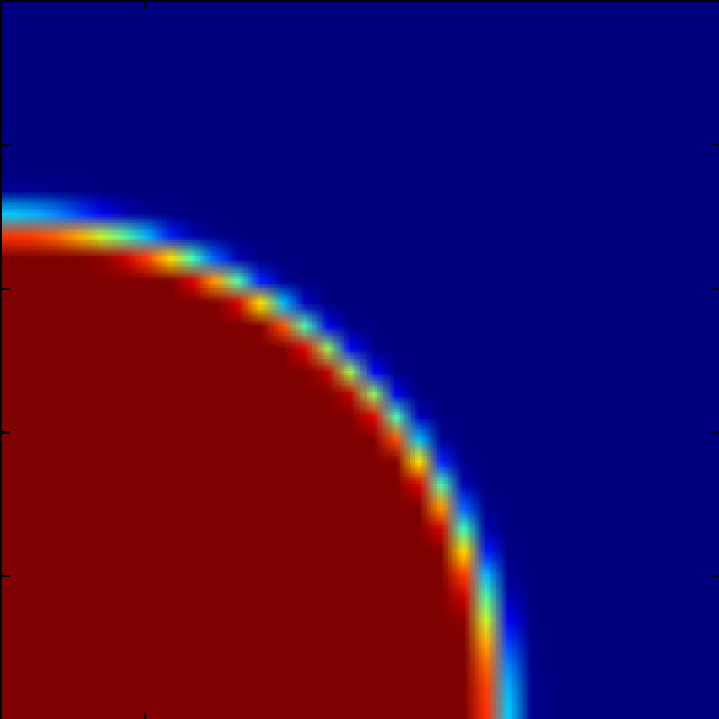
\includegraphics[scale=0.3]{i1-HIIcontour_100myr_nx32.eps}
  %% \hspace{0.1cm}
  %% 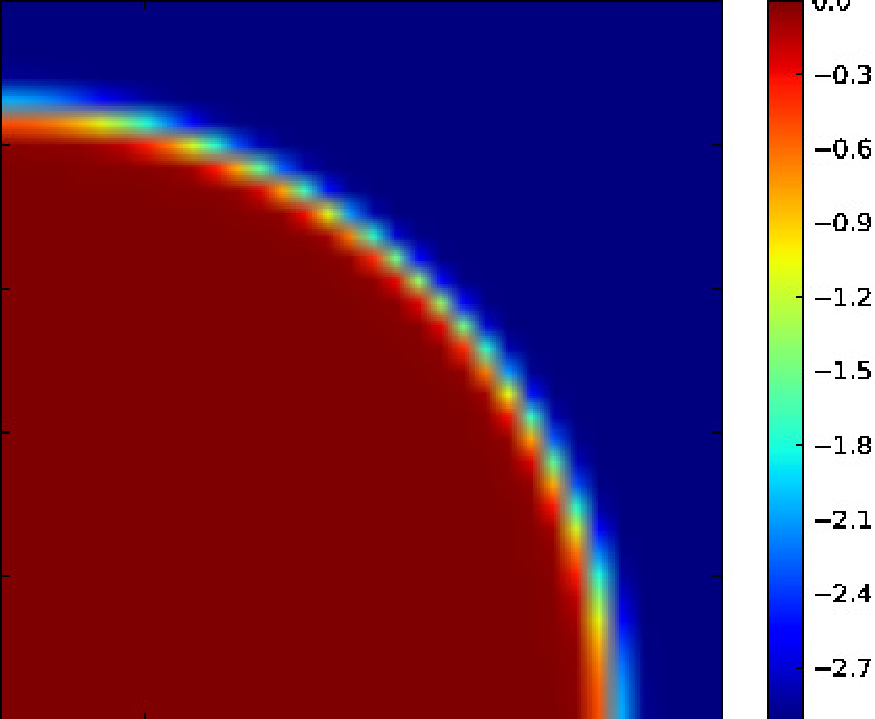
\includegraphics[scale=0.3]{i1-HIIcontour_500myr_nx32.eps}
  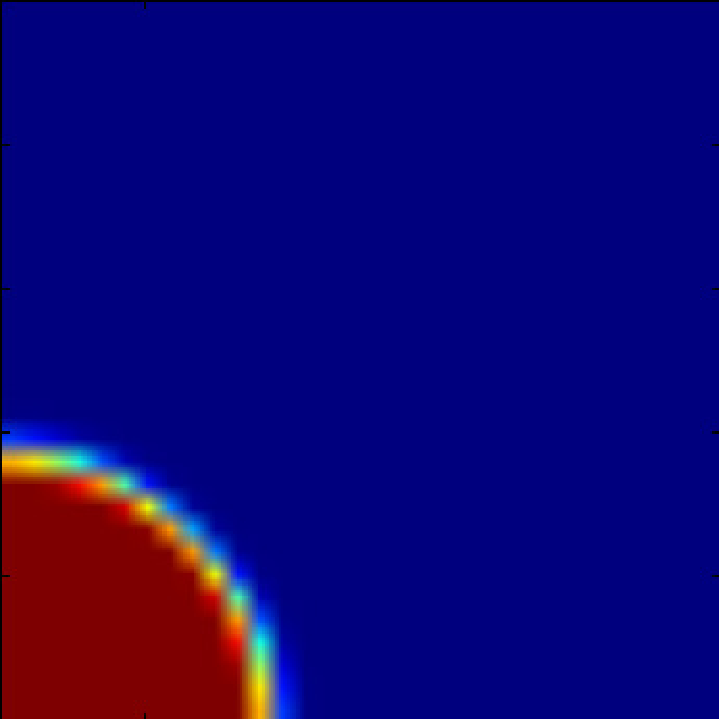
\includegraphics[scale=0.3]{i1-HIIcontour_10myr_nx32.pdf}
  \hspace{0.1cm}
  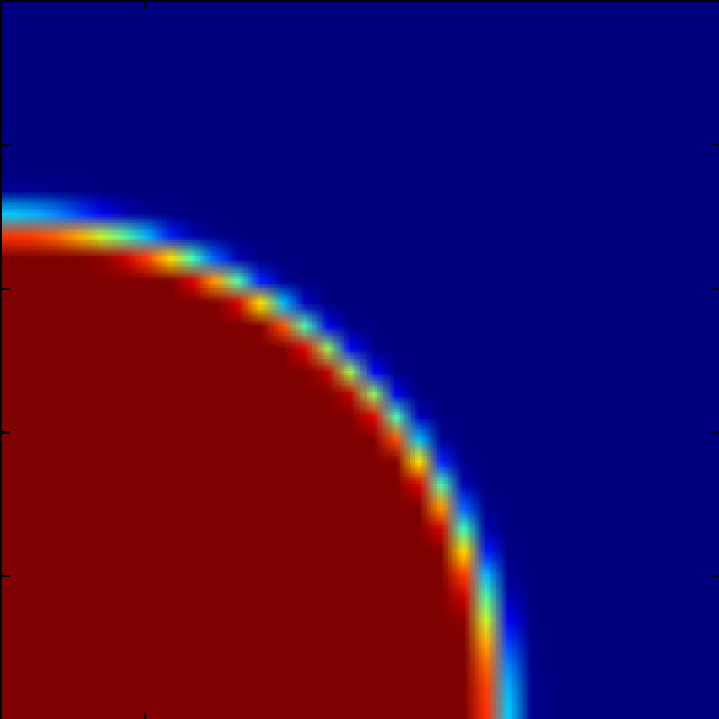
\includegraphics[scale=0.3]{i1-HIIcontour_100myr_nx32.pdf}
  \hspace{0.1cm}
  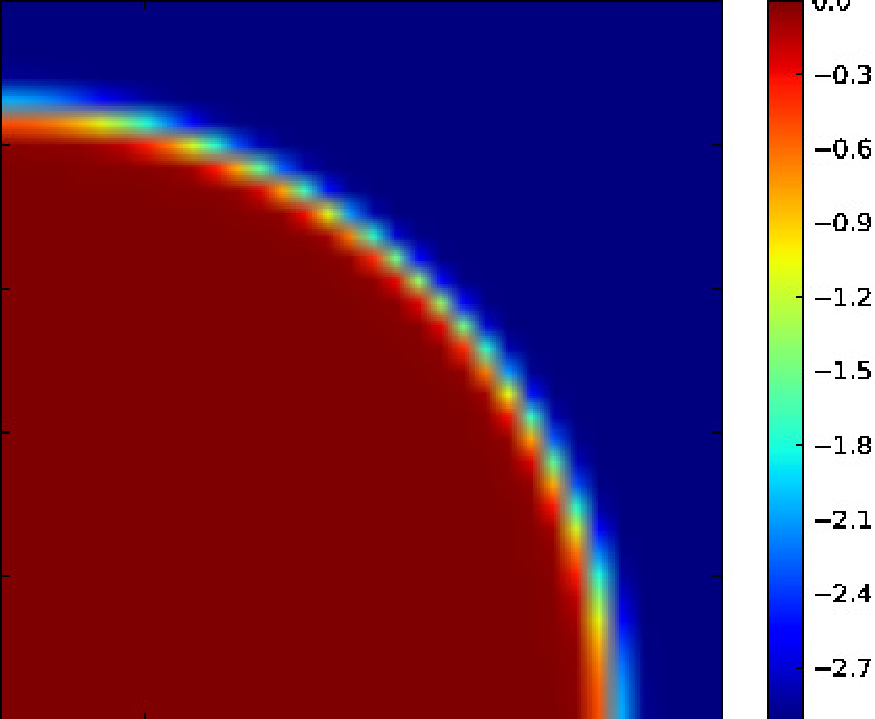
\includegraphics[scale=0.3]{i1-HIIcontour_500myr_nx32.pdf}
  \hfill}
\vspace{0.2cm}
\centerline{\hfill
  %% 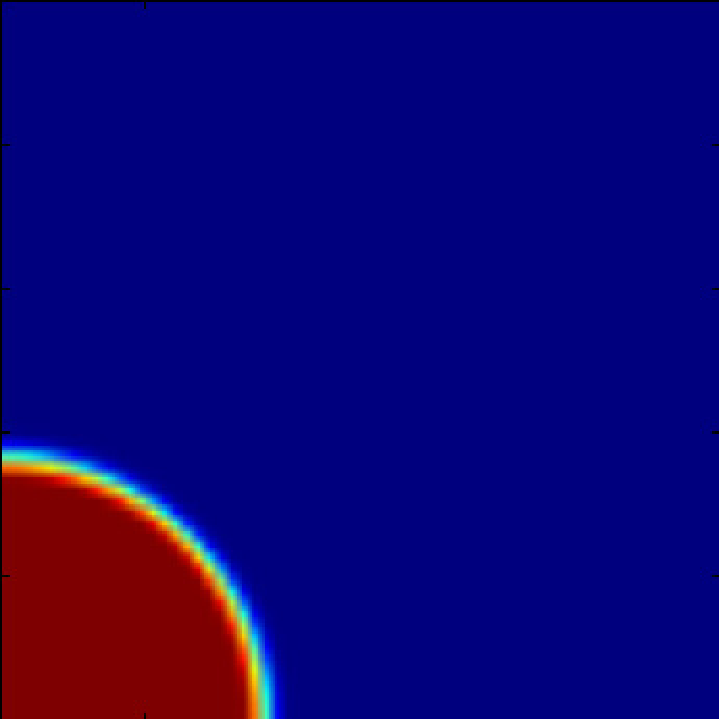
\includegraphics[scale=0.3]{i1-HIIcontour_10myr_nx64.eps}
  %% \hspace{0.1cm}
  %% 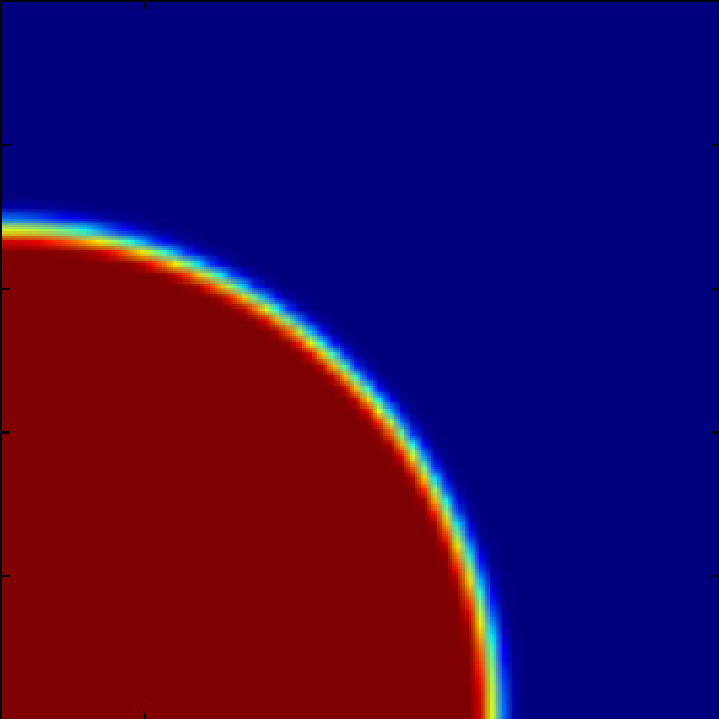
\includegraphics[scale=0.3]{i1-HIIcontour_100myr_nx64.eps}
  %% \hspace{0.1cm}
  %% 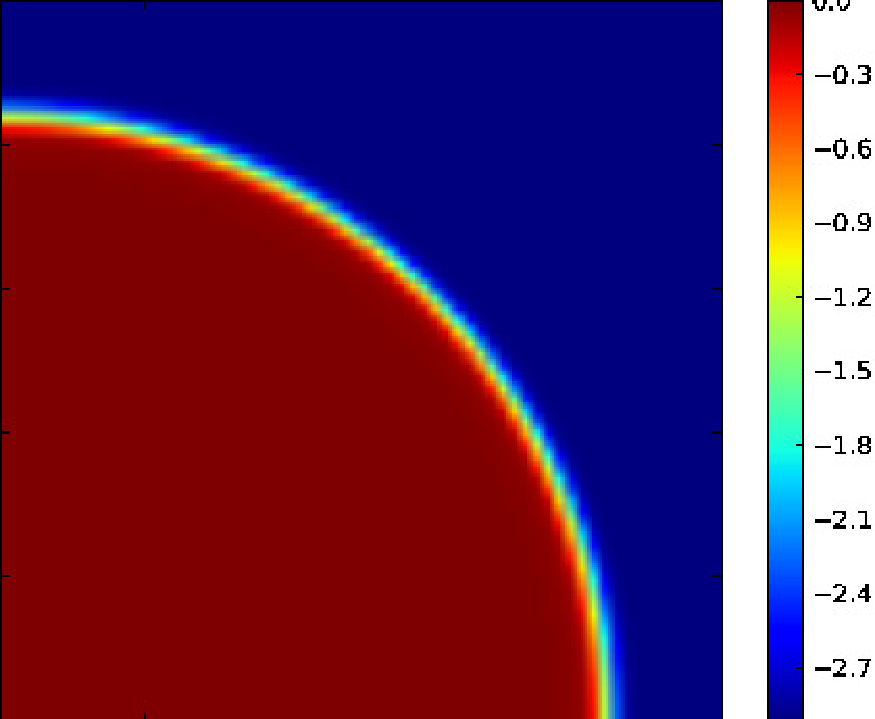
\includegraphics[scale=0.3]{i1-HIIcontour_500myr_nx64.eps}
  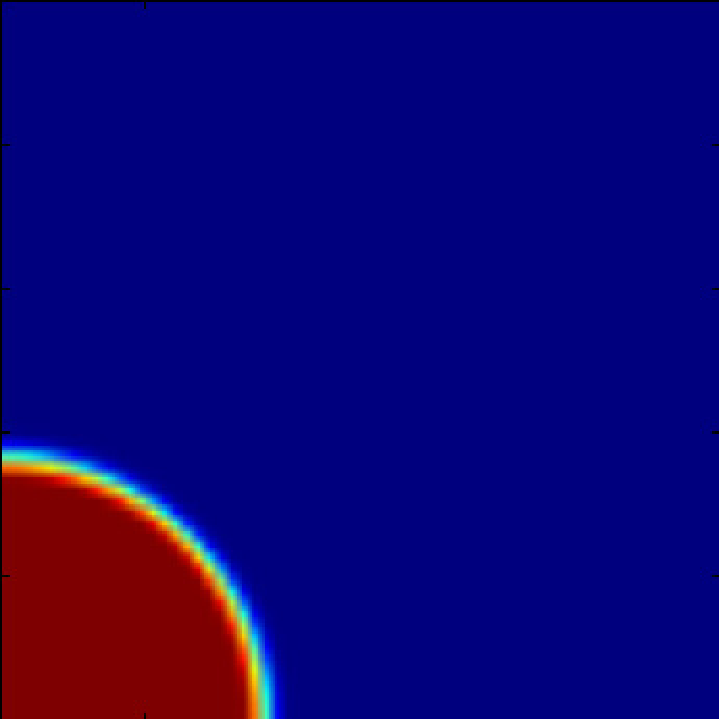
\includegraphics[scale=0.3]{i1-HIIcontour_10myr_nx64.pdf}
  \hspace{0.1cm}
  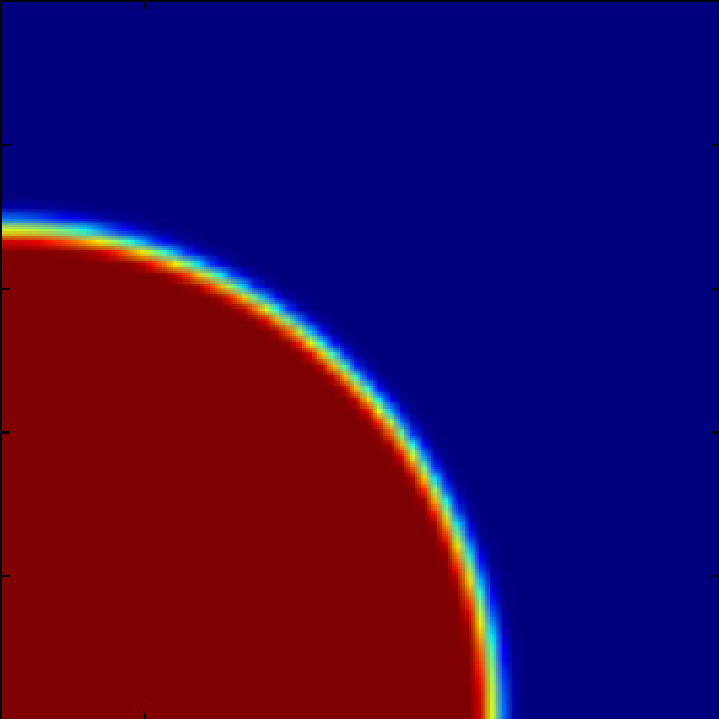
\includegraphics[scale=0.3]{i1-HIIcontour_100myr_nx64.pdf}
  \hspace{0.1cm}
  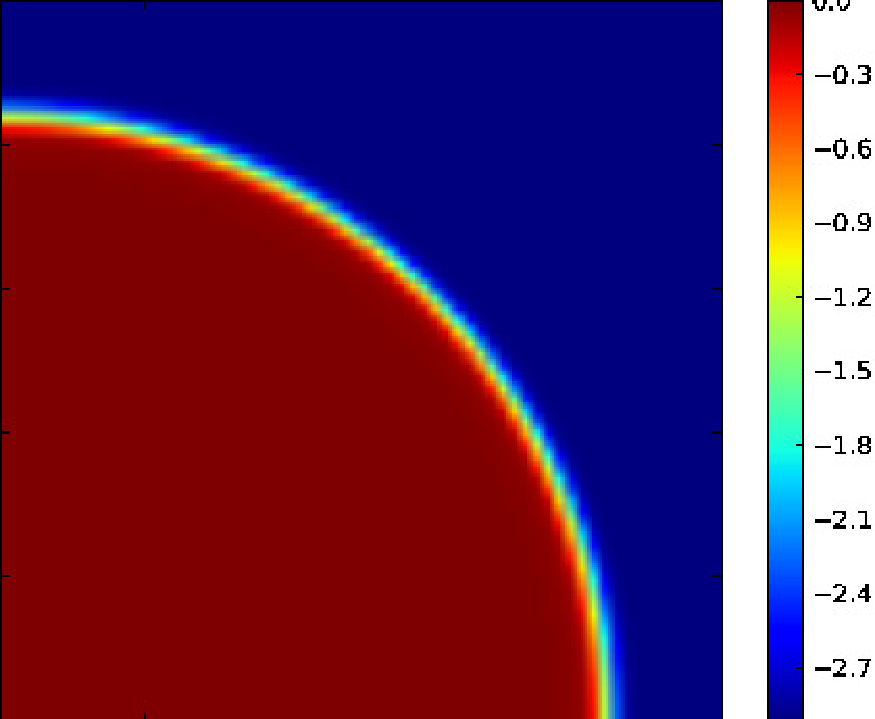
\includegraphics[scale=0.3]{i1-HIIcontour_500myr_nx64.pdf}
  \hfill}
\vspace{0.2cm}
\centerline{\hfill
  %% 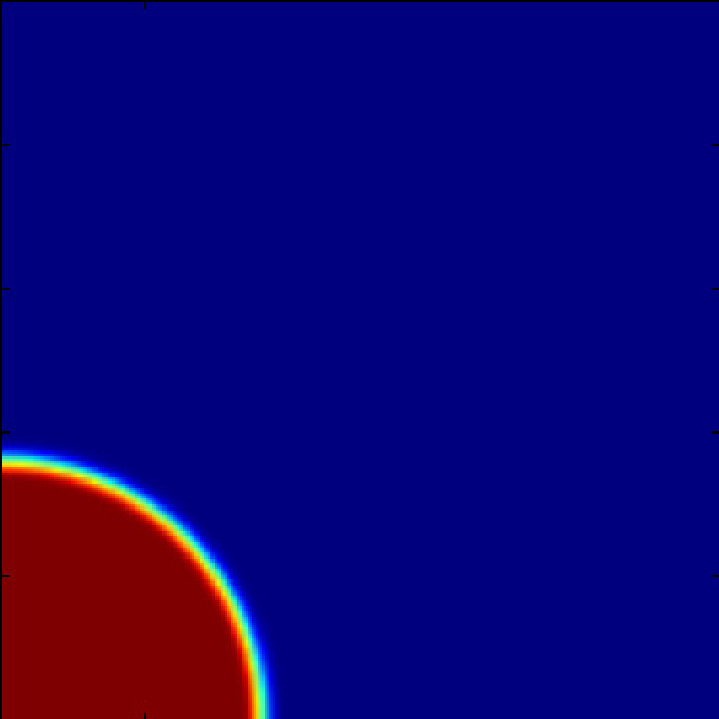
\includegraphics[scale=0.3]{i1-HIIcontour_10myr_nx128.eps}
  %% \hspace{0.1cm}
  %% 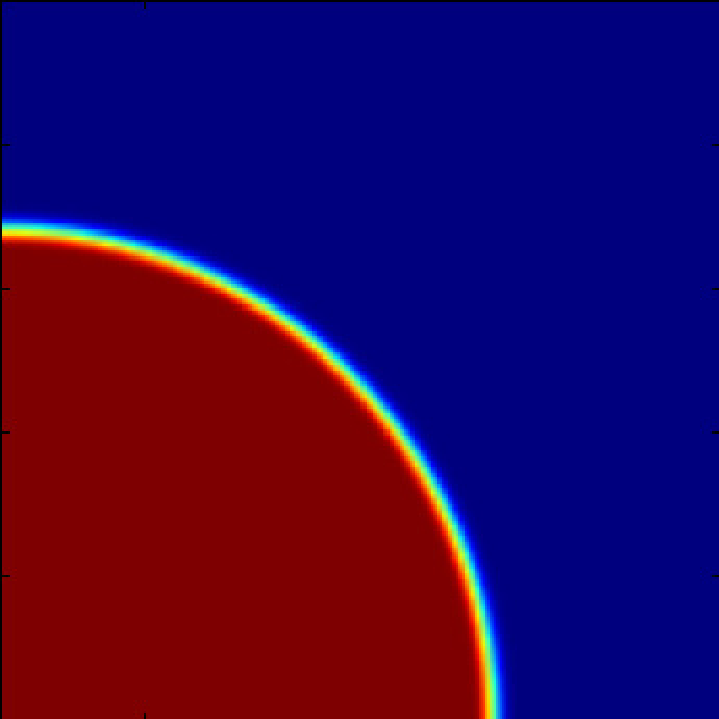
\includegraphics[scale=0.3]{i1-HIIcontour_100myr_nx128.eps}
  %% \hspace{0.1cm}
  %% 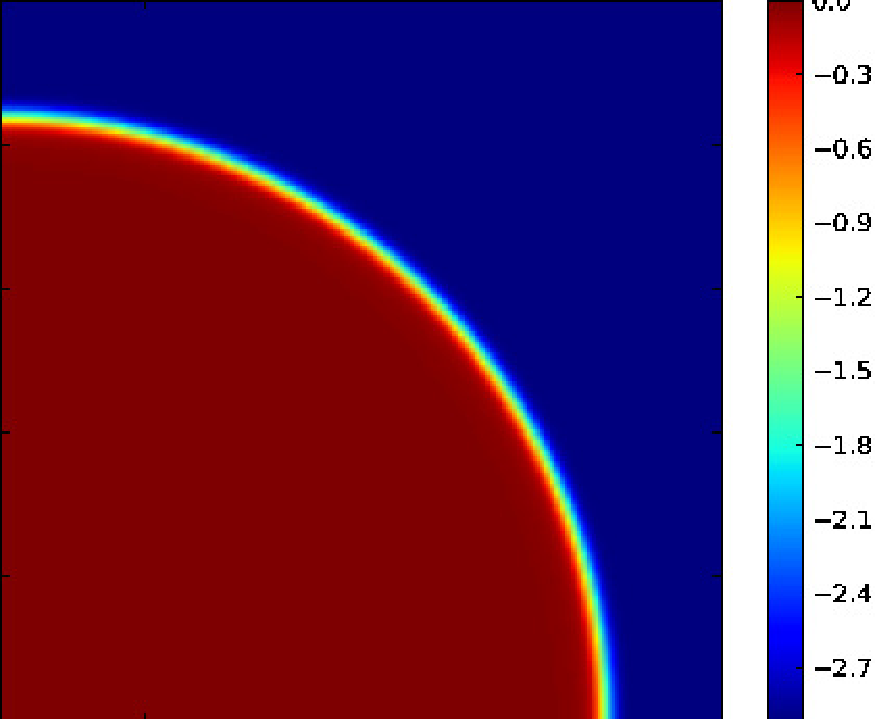
\includegraphics[scale=0.3]{i1-HIIcontour_500myr_nx128.eps}
  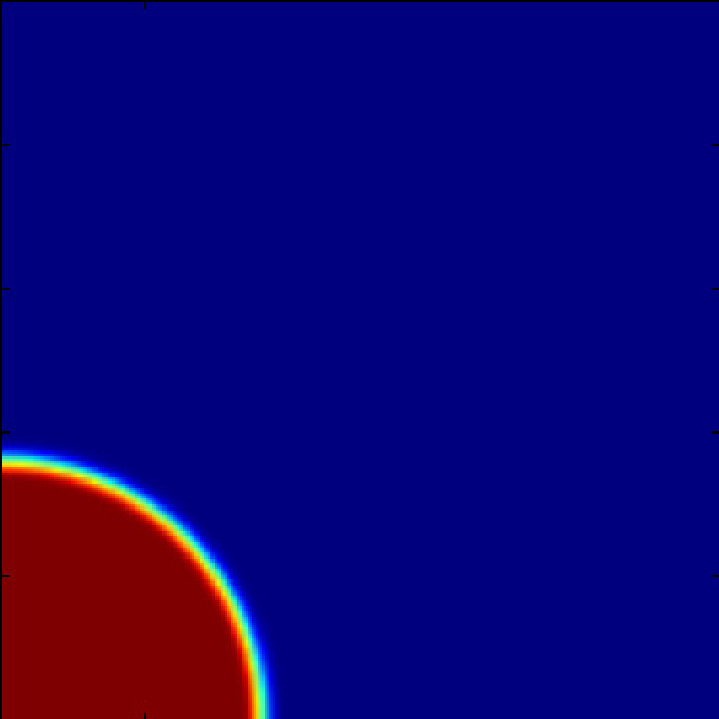
\includegraphics[scale=0.3]{i1-HIIcontour_10myr_nx128.pdf}
  \hspace{0.1cm}
  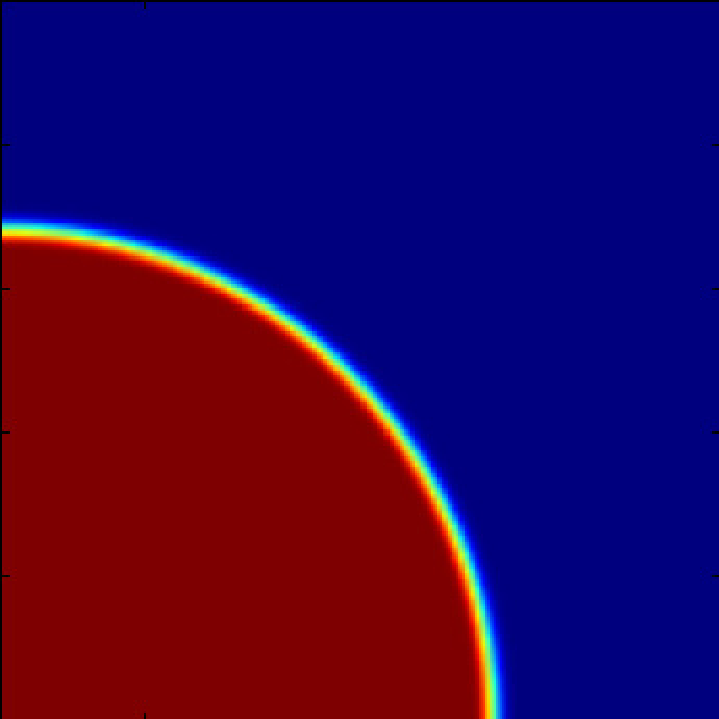
\includegraphics[scale=0.3]{i1-HIIcontour_100myr_nx128.pdf}
  \hspace{0.1cm}
  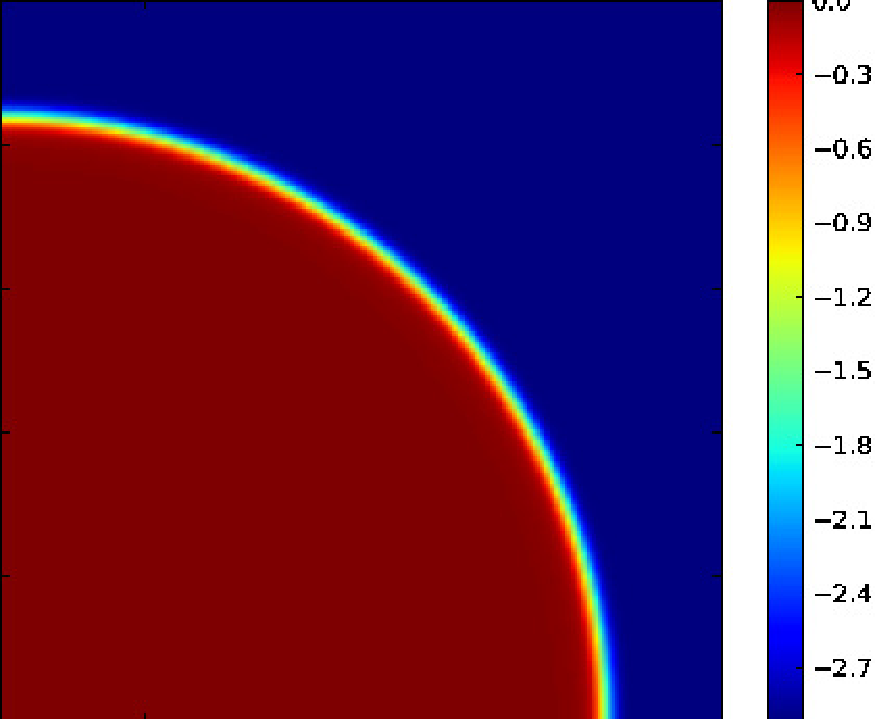
\includegraphics[scale=0.3]{i1-HIIcontour_500myr_nx128.pdf}
  \hfill}
  \caption{HII slices perpendicular to the $z$ axis (log$_{10}$
    scale).  We plot the evolution of the ionized region at times of
    10, 100 and 500 Myr (columns), and using spatial meshes of $16^3$,
    $32^3$, $64^3$ and $128^3$ (rows), to demonstrate the convergence
    to a spherical bubble.}
  \label{fig:i1_contours}
\end{figure}


\subsubsection{Cosmological radiative ionization}
\label{subsec:test2}

This verification test is a slight variation of the previous problem,
adding only the additional complication of a cosmologically expanding
universe.  Due to the cosmological expansion, the Str{\"o}mgren radius
itself increases due to the expansion of space, that reduces the
hydrogen number density $n_H$ as time proceeds,
\begin{equation}
  \label{eq:rs_cosmo}
  r_s(t) = \left(\frac{3\,\dot{N}_{\gamma}}{4\pi\,\alpha_B\,n_H(t)^2}\right)^{1/3}.
\end{equation}
This causes the I front to initially approach $r_s$, but eventually
fall behind as the expansion drives $r_s$ outward.  The analytical
solution to this problem is given by \cite{ShapiroGiroux1987},
\begin{align}
  \label{eq:radius_cosmo}
  r(t) &= r_{s,0} \left(\lambda e^{-\tau(a(t))} \int_{1}^{a(t)}
    e^{\tau(\tilde{a})}\left(1-2q_0+\frac{2q_0}{\tilde{a}}(1-z_0)\right)^{-1/2}\,\mathrm
    d\tilde{a} \right)^{1/3}, \\
  \notag \mbox{where} \qquad & \\
  \label{eq:tau}
  \tau(a) &= \lambda\left(F(a) - F(1)\right) \left(6q_0^2(1+z_0)^2\right)^{-1}, \\
  \label{eq:Fa}
  F(a) &= \left(2 - 4q_0 - \frac{2q_0}{a}(1+z_0)\right) 
     \left(1-2q_0+\frac{2q_0}{a}(1+z_0)\right)^{1/2}.
\end{align}
Here, the parameter $\lambda = \alpha_B n_{H,0} / H_0 / (1+z_0)$, with
$r_{s,0}$, $z_0$ and $n_{H,0}$ as the Str{\"o}mgren radius, redshift
and hydrogen number density at the beginning of the simulation.
Additionally, $q_0$ is the cosmological deceleration parameter, $H_0$
is the Hubble constant, and $a(t) = (1+z(t))^{-1}$ is the cosmological
expansion parameter. 

We run this problem using the parameters $q_0 = 0.5$, 
domain $[0,80\,\mbox{kpc}]^3$ (comoving), time/redshift domain $z =
[4,0]$, $H_0=0.5$, energy density contributions $\Omega_m = 1$,
$\Omega_A = 0$ and $\Omega_b = 0.2$.  Our initial conditions are $\rho
= 1.175\times 10^{-28}$ g cm$^{-3}$, $T = 10^4$ K and $E = 10^{-45}$
erg cm$^{-3}$.

We again plot spherically-averaged radial profiles of the radiation energy
density and the ionization fractions at redshifts 3.547, 2.423 and 1.692 from a
simulation using a 128$^3$ spatial grid and time step tolerance
$\tau_{tol} = 10^{-4}$ in Figure \ref{fig:sg_results}, showing the
expected propagation and eventual stalling of the radiation front and
resulting I-front in time.
\begin{figure}[t]
\centerline{\hfill
  %% 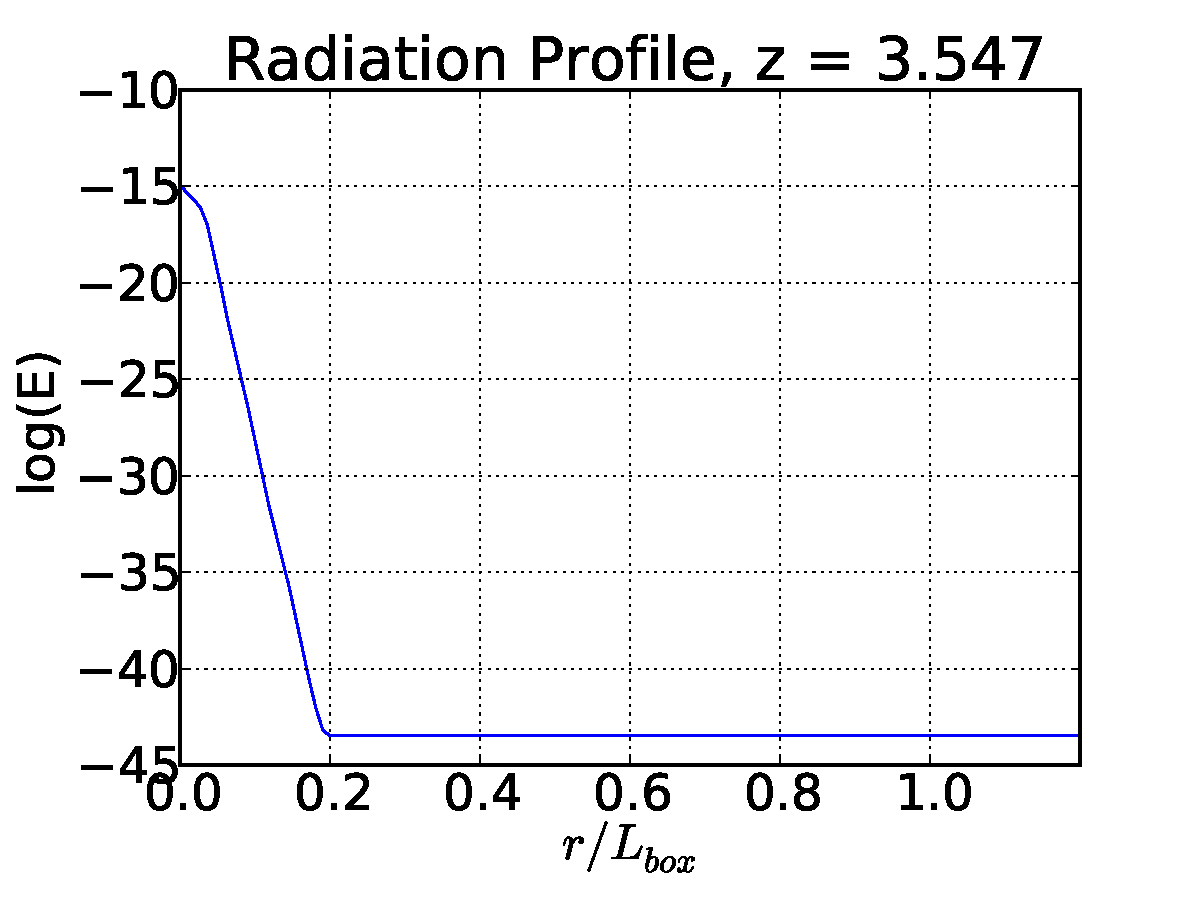
\includegraphics[scale=0.3, trim=1.0cm 0.5cm 1.0cm 0.5cm]{sg-Eprofiles_01.eps}
  %% 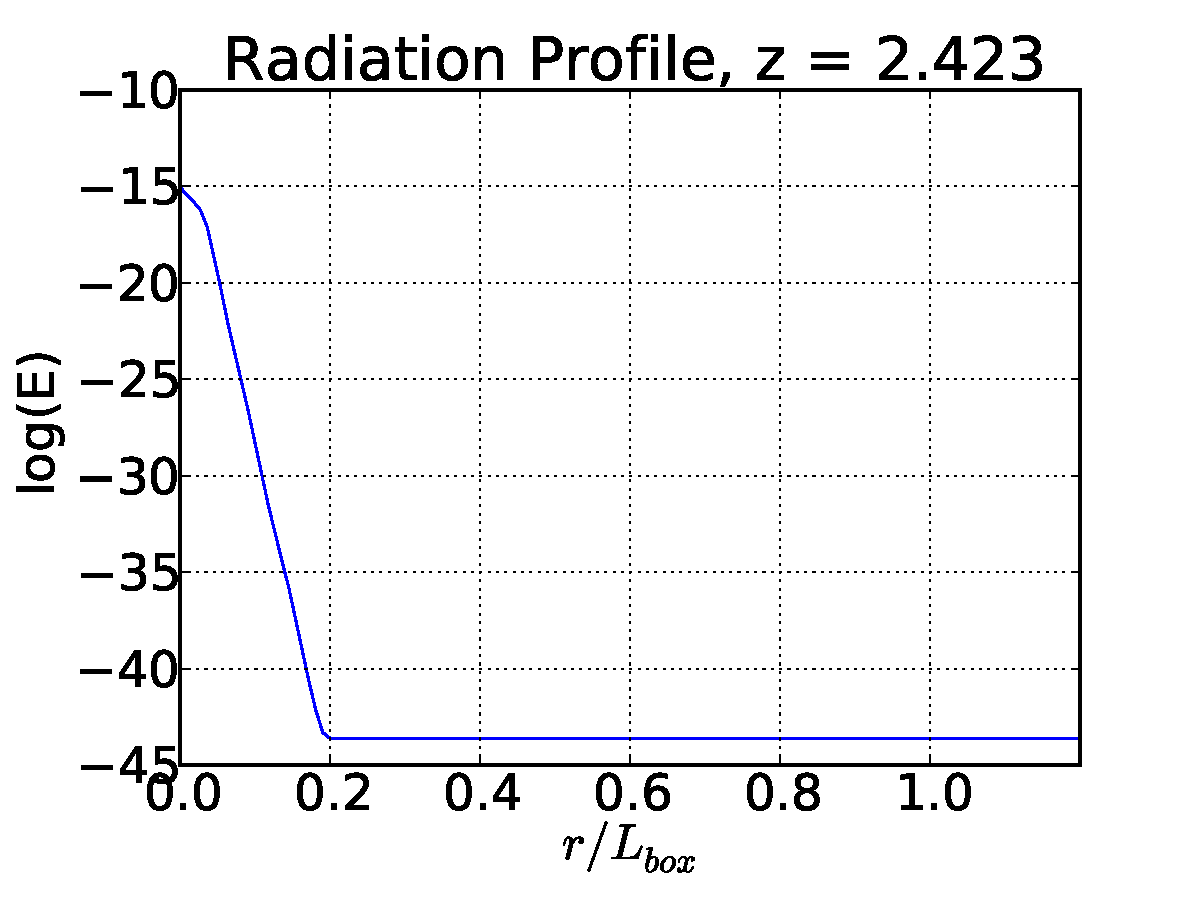
\includegraphics[scale=0.3, trim=1.0cm 0.5cm 1.0cm 0.5cm]{sg-Eprofiles_05.eps}
  %% 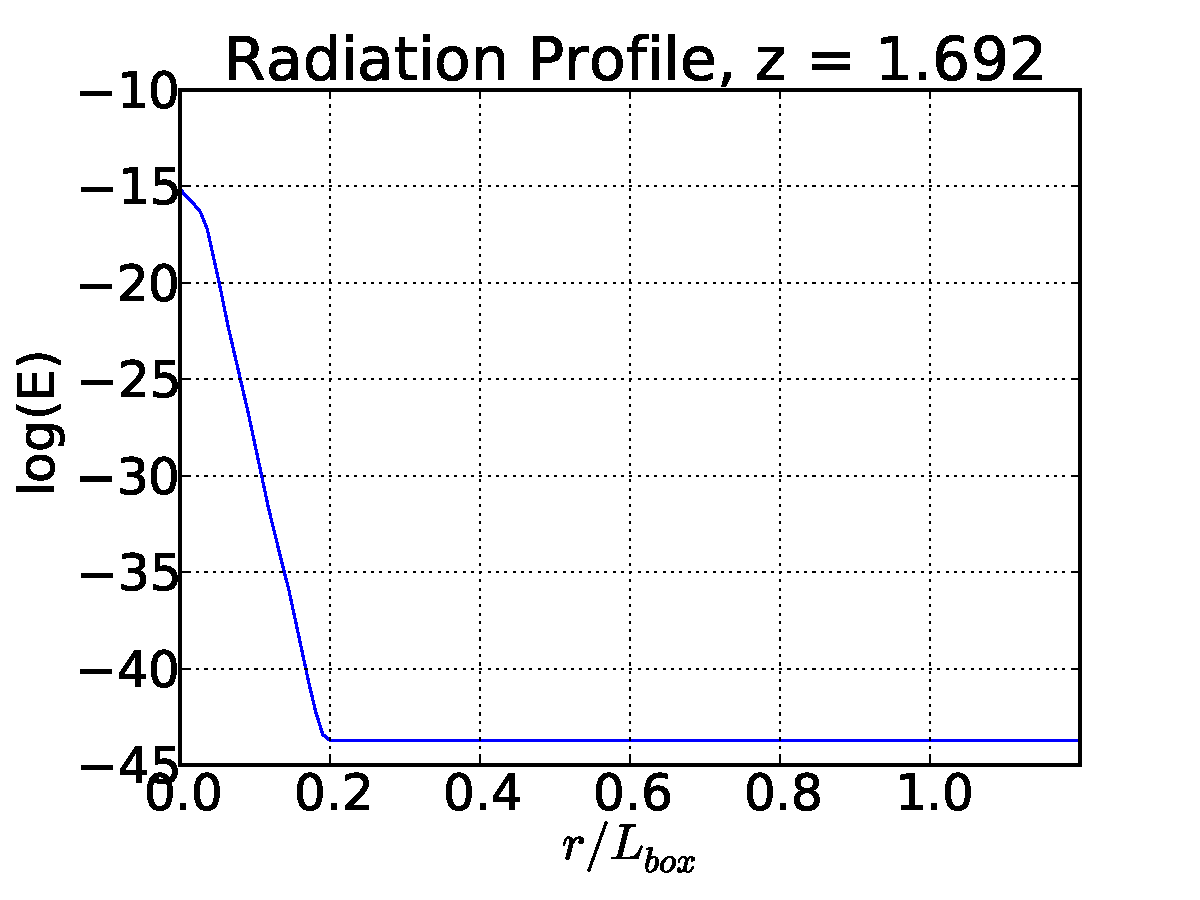
\includegraphics[scale=0.3, trim=1.0cm 0.5cm 1.0cm 0.5cm]{sg-Eprofiles_10.eps}
  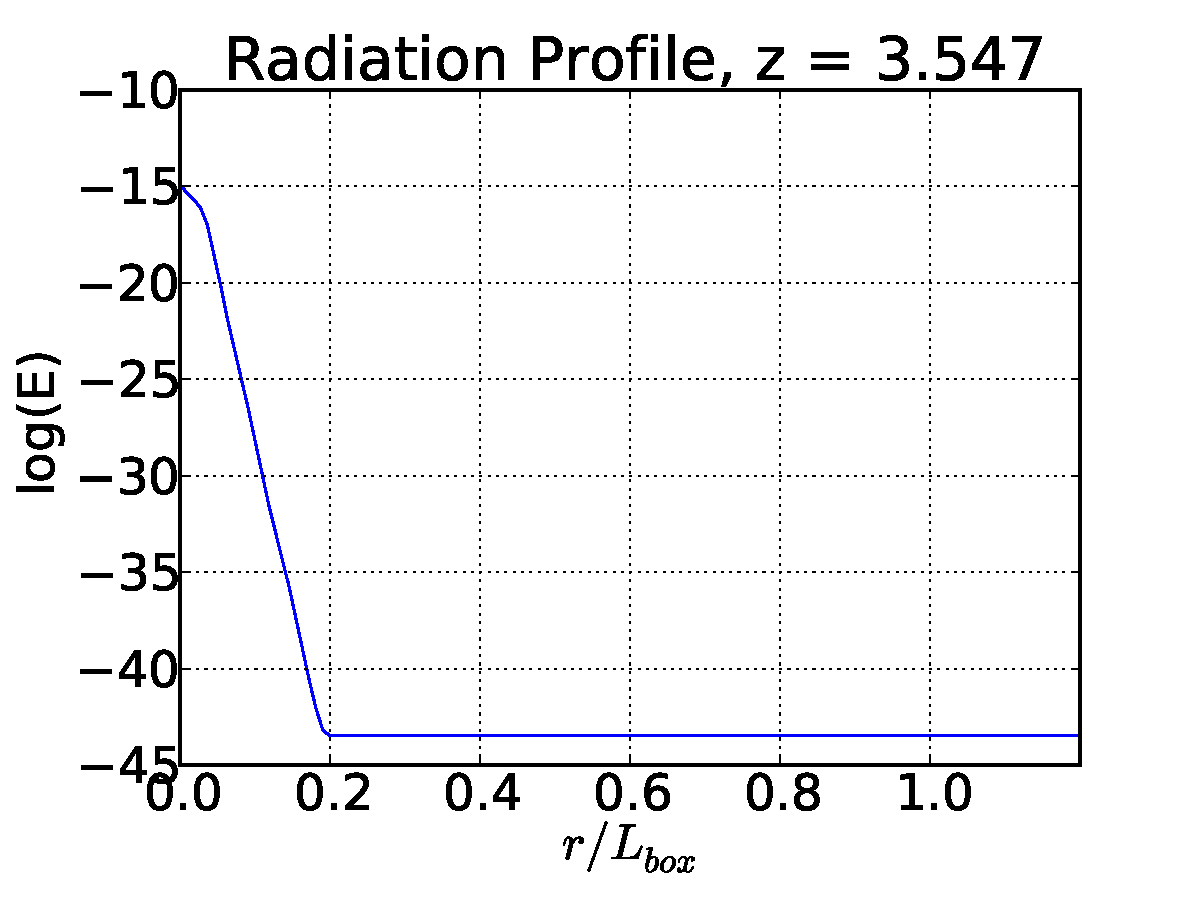
\includegraphics[scale=0.3, trim=1.0cm 1.0cm 1.0cm 0.5cm]{sg-Eprofiles_01.pdf}
  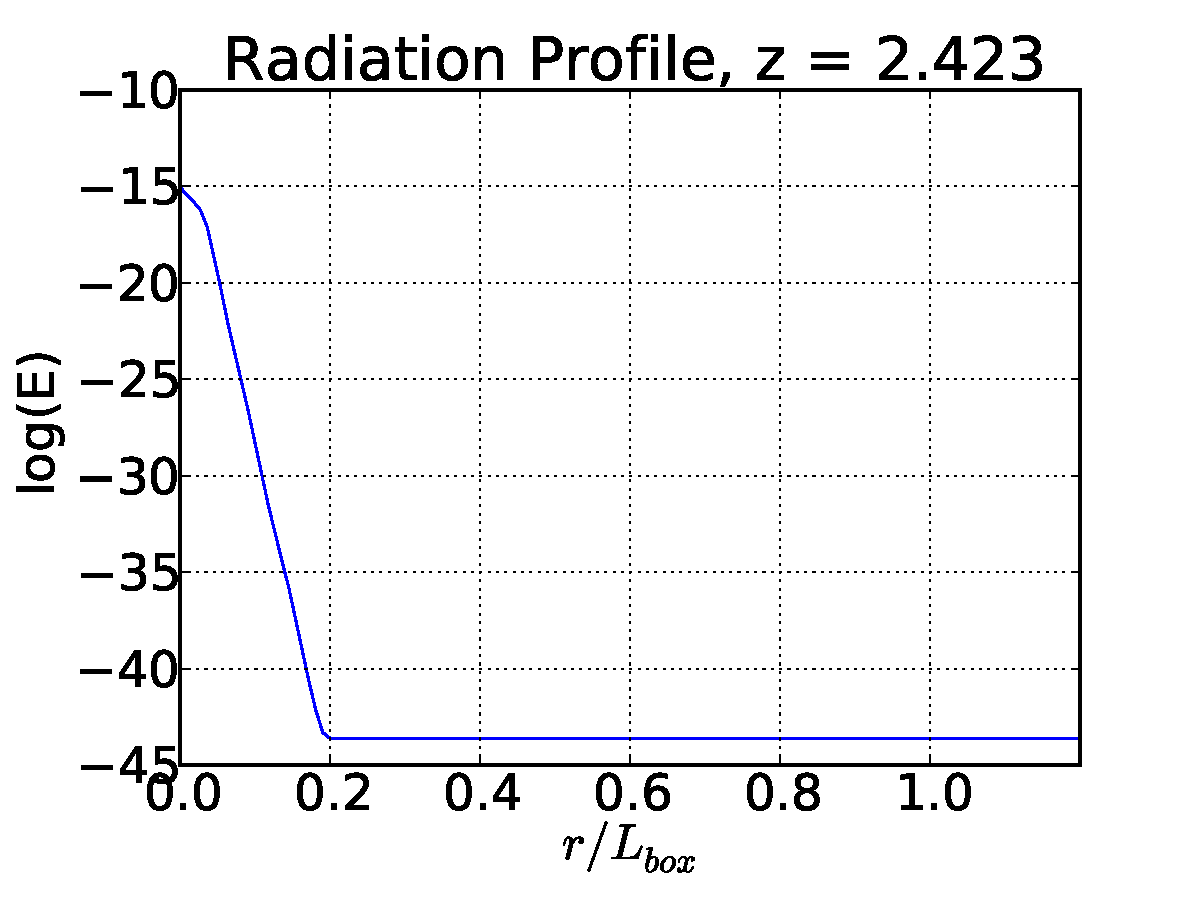
\includegraphics[scale=0.3, trim=1.0cm 1.0cm 1.0cm 0.5cm]{sg-Eprofiles_05.pdf}
  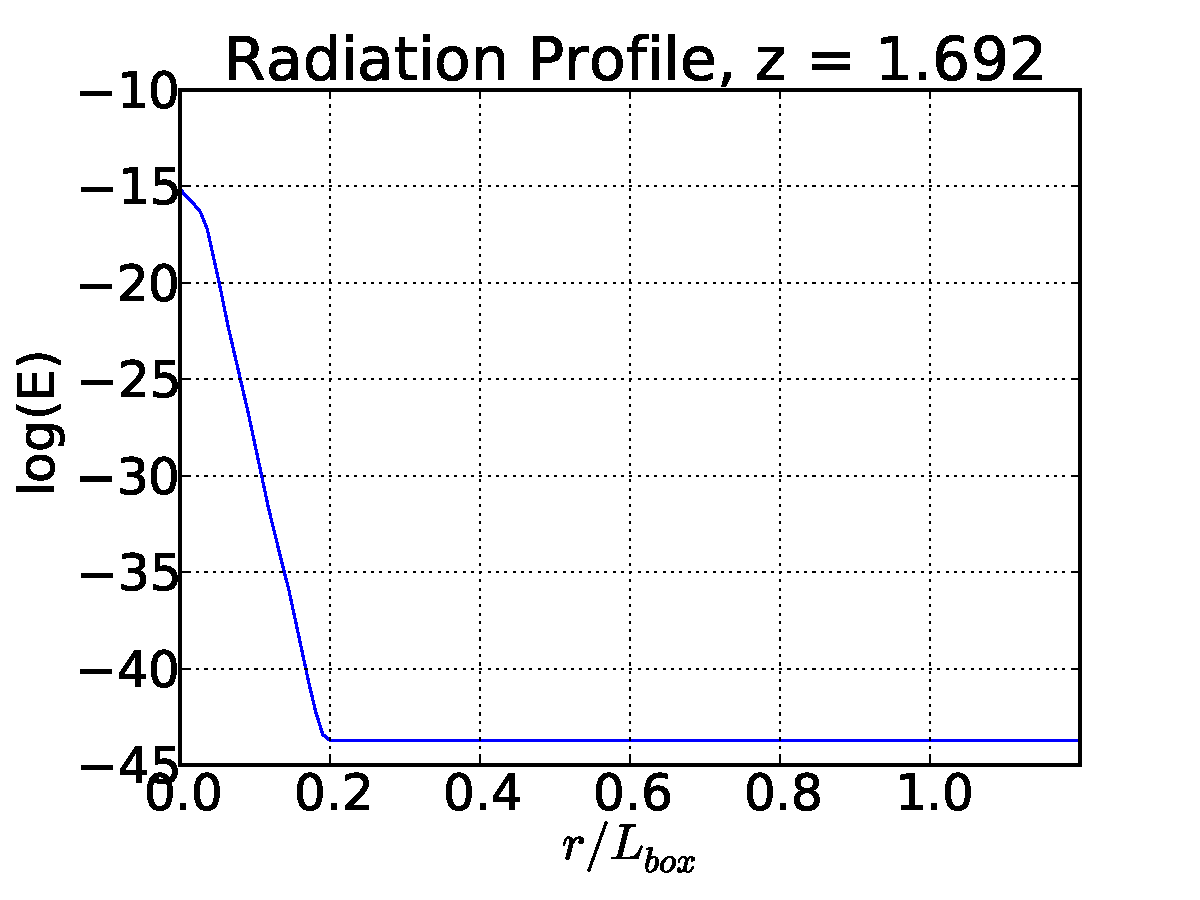
\includegraphics[scale=0.3, trim=1.0cm 1.0cm 1.0cm 0.5cm]{sg-Eprofiles_10.pdf}
  \hfill}
\centerline{\hfill
  %% \includegraphics[scale=0.3, trim=1.0cm 0.5cm 1.0cm 0.5cm]{sg-profiles_01.eps}
  %% \includegraphics[scale=0.3, trim=1.0cm 0.5cm 1.0cm 0.5cm]{sg-profiles_05.eps}
  %% \includegraphics[scale=0.3, trim=1.0cm 0.5cm 1.0cm 0.5cm]{sg-profiles_10.eps}
  \includegraphics[scale=0.3, trim=1.0cm 0.5cm 1.0cm 0.5cm]{sg-profiles_01.pdf}
  \includegraphics[scale=0.3, trim=1.0cm 0.5cm 1.0cm 0.5cm]{sg-profiles_05.pdf}
  \includegraphics[scale=0.3, trim=1.0cm 0.5cm 1.0cm 0.5cm]{sg-profiles_10.pdf}
  \hfill}
  \caption{Spherically-averaged radial profiles of radiation energy
    density and ionization fractions for the cosmological ionization
    test in section \ref{subsec:test2} using a $128^3$ mesh and
    time step tolerance $\tau_{tol} =10^{-4}$.  Plots are shown at z=3.547, 2.423 and 1.692
    (left to right), with the radiation energy density on
    the top row and ionization fractions on the bottom row.}
  \label{fig:sg_results}
\end{figure}
As with the previous test, we investigated the accuracy of our new
splitting approach between the radiation and chemistry solvers using
the same set of mesh sizes and time step tolerances as the test in
section \ref{subsec:test1}.  Figure \ref{fig:sg_stats} contains the
corresponding plots of the solution error and total runtime as a
function of the average time step size.  
\begin{figure}[t]
\centerline{\hfill
  %% \includegraphics[scale=0.45, trim=1.0cm 0.5cm 1.0cm 0.5cm]{sg-error_enzo.eps}
  %% \includegraphics[scale=0.45, trim=1.0cm 0.5cm 1.0cm 0.5cm]{sg-runtime_enzo.eps}
  \includegraphics[scale=0.45, trim=1.0cm 0.0cm 1.0cm 0.5cm]{sg-error_enzo.pdf}
  \includegraphics[scale=0.45, trim=1.0cm 0.0cm 1.0cm 0.5cm]{sg-runtime_enzo.pdf}
  \hfill}
  \caption{We ran tests using mesh sizes of
    $16^3$, $32^3$ and $64^4$, and time step tolerances of
    $10^{-2}$, $10^{-3}$, $10^{-4}$ and $10^{-5}$, and plot the I
    front position error as a function of the average time step size.
    As with Figure \ref{fig:i1_stats}, the runtime scales linearly
    with the inverse $\Delta t_{avg}$, and the error scales linearly
    with $\Delta t_{avg}$, at least until other sources of error
    dominate the calculation.} 
  \label{fig:sg_stats}
\end{figure}
Our results are similar to those from the previous test, indicating
that the modified time evolution approach employed in this work
successfully achieves accurate solutions of our coupled radiation and
ionization system.



\subsection{Validation Tests}
{\bf Validation tests are tests without analytic solutions that nonetheless serve as a
useful point of comparison between codes implementing different physical 
models and numerical methods \citep{IlievEtAl2006,IlievEtAl2009}. Our purpose is not to run all possible tests, but rather to validate the application of FLD to large scale reionization simulations, and in particular to investigate the well-known inability of FLD to cast a shadow on the general progress of reionization.
In this section we test our algorithm against 
four validation tests that are most relevant to the problem of cosmological 
reionization. The first two are radiation hydrodynamic tests studied by \cite{IlievEtAl2009} (hereafter RT09). They are the propagation of an I-front in a $r^{-2}$ density gradient, and the photoevaportion of a dense cloud irradiated from one side. The third validation test is the consolidated \hii region produced by two sources of equal luminosity introduced by \cite{Petkova09}. These three tests were chosen from a larger number of tests in the literature because they form a natural sequence with regard to the expansion and merging of isolated \hii regions in a clumpy IGM.  Finally, in a fourth test of our own design, we perform a direct comparison between FLD and ray tracing on a fully coupled reionization simulation in a small box. These tests demonstrate that although FLD ionizes dense clouds somewhat faster than methods that cast shadows, this affects primarily the earliest phases of cosmic reionzation when  a piece of neutral IGM is irradiated by the brightest nearby source. Later on, when multiple sources ionize the gas from multiple directions, FLD and ray tracing produce very similar evolutions. }    \st{To our knowledge these are the first FLD results
published to date, since the other codes running these problems have
focused on ray-tracing, Monte Carlo, and variable tensor Eddington
approximations of the radiative transfer equations.} 





\subsubsection{Test 6 -- I-front expansion in a $r^{-2}$ density profile}
\label{subsec:test6}

{\bf As our first validation test, we investigate Test 6 in
\cite{IlievEtAl2009} (hereafter RT09), that focuses on a full
radiation-hydrodynamics simulation of an ionized hydrogen (HII)
region in a spherically-symmetric density field.  Here, the center of
the region has constant number density, but at a specified core radius
$r_0$ the density rapidly decreases with radius.  Denoting this
functional relationship as $n_H(r)$, 
\[
   n_H(r) = \begin{cases}
     n_0,\quad&\text{for}\; r\le r_0\\
     n_0\left(\frac{r_0}{r}\right)^{2},\quad&\text{for}\; r> r_0.
   \end{cases}
\]
We follow the parameters choices from \cite{IlievEtAl2009}:  cubic
simulation domain of $[0,L]^3$ with $L=0.8$ kpc, core number density
$n_0 = 3.2$ cm$^{-3}$, core radius $r_0 = 91.5$ pc, zero initial
ionization fraction, ionization source at the origin with strength
$\dot{N}_{\gamma}=10^{50}$ photons s$^{-1}$ and a $T=10^5$ K blackbody
SED, initial temperature $T = 100$ K, reflective boundaries that touch
the origin and transmissive boundaries elsewhere, and a total
simulation time of $0\le t\le 25$ Myr.  Under these choices the
the I-front transitions from R-type to D-type within the core.  Once
the I-front reaches the beginning of the density gradient it begins to
accelerate, subsequently transitioning back to R-type.  Unfortunately,
for these simulation parameters, the problem exhibits no analytical
solution, so we refer to RT09 and WA11 for reference solutions to
compare against our own.

In the left half of Fig.~\ref{fig:test6_plots} we show time histories
of the I-front radius and velocity, that exhibit strong agreement with
the results from both RT09 and WA11.  In the right half of 
Fig.~\ref{fig:test6_plots} we plot radial profiles of the number
density, temperature, ionized fraction and pressure in the simulation
at 3, 10 and 25 Myr.  All of these results agree with reference
results from RT09 and WA11.  Perhaps the most notable difference may
be seen in the temperature and pressure profiles in comparison with
WA11, where our use of a grey approximation does not capture gas
preheating ahead of the I-front.

In Fig.~\ref{fig:test6_slices} we plot slices through the origin
of the ionized fraction, neutral fraction, temperature and number
density in the simulation at 25 Myr.  As it evident in these plots,
the FLD radiation approximation maintains a nearly spherical solution
profile throughout the simulation, with a slight anisotropy in the
non-coordinate aligned directions.  However, even with this minor
deviation of spherical symmetry, the results compare well against the
those in RT09 and WA11, many of which exhibit much more significant
anisotropy than that shown here. }



\begin{figure}[t]
\centerline{\hfill
  \includegraphics[scale=0.42, trim=0.0cm 0.0cm 0.0cm 0.0cm]{test6_radius.pdf}
  \includegraphics[scale=0.42, trim=0.0cm 0.0cm 0.0cm 0.0cm]{test6_profiles.pdf}
  \hfill}
  \caption{Test 6 (HII region in a $r^{-2}$ density profile).  Top
    left: growth of the computed I-front radius, computed as the
    radius with 50\% ionized fraction.  Bottom left: velocity of
    I-front radius, as computed from the upper plot at 0.5 Myr
    intervals.  Right: radial profiles at 3, 10 and 25 Myr, clockwise
    from top left as number density, temperature, pressure and Mach
    number.} 
  \label{fig:test6_plots}
\end{figure}

\begin{figure}[t]
\centerline{\hfill
  \includegraphics[scale=0.42, trim=0.0cm 0.0cm 0.0cm 0.0cm]{test6_slices.pdf}
  \hfill}
  \caption{Test 6 (HII region in a $r^{-2}$ density profile). Slices
    through the origin at 25 Myr.  Clockwise from top left: ionized
    fraction, Mach number, temperature and number density.}
  \label{fig:test6_slices}
\end{figure}






\subsubsection{Test 7 -- Photoevaporation of a dense clump}
\label{subsubsec:test7}
As our {\bf second} validation test we run Test 7 of RT09, and also studied by WA11 using {\em Enzo+Moray}. 
This is a radiation hydrodynamic test involving ionizing radiation impinging on a dense, opaque spherical cloud
which is subsequently photoevaporated. RT09 set this up as a plane wave of ionizing radiation sweeping over the 
cloud, {\bf whereas WA11 illuminated the cloud with a single point source whose luminosity was adjusted to produce the same ionizing flux at the cloud.} To facilitate comparison with the RT09 results, {\bf we implement the plane-wave illumination scheme, as described below} \st{we set it up as a spherical wave of ionizing radiation from
a point source sweeping over the cloud.} If run without hydrodynamics, the I-front is trapped in the dense cloud,
and the cloud casts a sharp shadow {\bf \citep{IlievEtAl2006}.  In reality, recombination radiation which would partially fill in the shadow zone, but this effect has not been included in validation tests to date. } With hydrodynamics engaged, the side of the cloud facing the source photoheats and expands, permitting a deeper
penetration of radiation into the cloud. Eventually, the entire cloud is photoevaporated. {\bf It is important to check
what FLD will do in this circumstance, in particular how the lack of a shadow affects the
photoevaporation time for the cloud.} \st{As we will now show, the effect is weak, validating our use of FLD for
large scale reionization problems.} 

The setup is as follows. A cubic domain 6.6 kpc on a side is employed, filled with an ambient medium of 
$n_H = 2 \times 10^{-4}$ cm$^{-3}$ and T=8000 K. The cloud is in pressure equilibrium with the intercloud
medium with density $n_H = 0.04$ cm$^{-3}$ and T=40 K. The cloud is a top-hat sphere with radius
$r_c$ = 0.8 kpc, and is centered at (x,y,z) = (5, 3.3, 3.3) kpc. The ionized fraction is initially zero everywhere. 
\st{A single radiation source is located in the center of the $x=0$ boundary. It has a luminosity of 
$\dot{N}_{\gamma}=3 \times 10^{51}$ photon/s.}
{\bf We implement the plane-wave illumination setup of RT09 by initializing an array of point sources on the left domain boundary, each emitting $10^6 A_{cell}$ ionizing photons/sec, where $A_{cell}$ is the area of the cell face. We have verified that this results in the correct flux of ionizing photons inside the domain.} \st{WA11 use the same four energy group spectral model to
represent a $10^5$ K blackbody as in Test 4 above. We use our grey FLD approximation which does not
model spectral hardening, as discussed above. We thus do not expect our results to be identical with WA11. }

Figs. \ref{fig:test7_slices_10} and \ref{fig:test7_slices_50}  shows slices through the cloud midplane of neutral fraction, pressure, temperature, and 
density at time $t=10, 50$ Myr, respectively. \st{At this time the I-front has propagated roughly 80\% through the cloud on the axis, compared to 
about 50\% in WA11. Because in the FLD approximation radiation propagates in the direction of the radiation energy density gradient,
it has filled in the  ``nightside" of the cloud, ionizing the cloud from all sides. By 10 Myr only a small neutral patch remains. 
Comparing with Fig. 27 
of WA11, we find similar structures on the ``dayside" of the cloud, but the complete absense of a neutral shadow on 
the nightside. }
{\bf By 10 Myr the cloud is fully ionized, whereas the results in RT09 show that the cloud is only partially ionized at this time. Inspection of Figs. 32 and 42 in RT09 suggest that the I front has only reached the center of the cloud after 10 Myr. The resolution of this discrepancy is that within the FLD approximation, the radiation quickly flows around the cloud, filling in the shadow region. The cloud is thus irradiated from all sides, not just one side. Therefore the time to ionize the cloud should be roughly the time it takes for the I-front to traverse a distance equal to the radius of the cloud. Ignoring attenuation, recombinations, and hydrodynamic effects the speed of the I-front in the dense gas is $v_{IF}=2.5 \times 10^7$ cm/s.  At this speed, it should take the I-front roughly 3.2 Myr to  reach the center of the cloud. }

{\bf In Fig. \ref{fig:time-evol} we plot the time evolution of the mass of \hi in the cloud. We see that the cloud becomes ionized on a timescale of about 5 Myr, somewhat longer than the estimate above. To improve on this estimate we ran a 1D version of the opaque cloud test. We placed a step function jump in density from $2 \times 10^{-4}$ cm$^{-3}$ to a value 200 times that at the center of the box; $x=3.3$ kpc. The position of the I-front versus time is shown in Fig. \ref{fig:box_wall_hydro-Ifront_history}. Including the attenuation of the ionizing flux, recombinations, and hydrodynamic motions, it takes the I-front about 5.8 Myr to propagate 0.8 kpc into the dense gas, in good agreement with Fig. \ref{fig:time-evol}.  }


%Fig. \ref{fig:test7_slices_50} shows the same information for the cloud at $t=50$ Myr.} 
By \st{this time} {\bf 50 Myr} the cloud has
expanded considerably and become completely ionized, exhibiting a roughly spherical shape. 
The results of {\bf RT09 and} WA11 are similar, except for a small wedge-shaped neutral patch on the back of the cloud, which casts 
a small shadow into the diffuse intercloud medium. 
In reality, ionizing recombination radiation from the denser cloud gas would fill in this shadow and ionize the 
diffuse gas there, making it more like the FLD solution. 

To enable a more quantitative comparison with {\bf RT09 and}  WA11,
we plot in Fig. \ref{fig:test7_profiles} line cuts from the point source through the center of the cloud at
$t=1, 10, 50$ Myr. 
Because the FLD method ionizes the cloud from all sides with only a small delay between
dayside and nightside irradiation, we see a less pronounced dayside-nightside asymmetry in the density and neutral fraction 
profiles compared with WA11 at 10 and 50 Myr. Both methods show good agreement on the position and structure
of the dense shell swept up by the expanding cloud at 50 Myr at $x/L_{box} \sim 0.4$. 
Significant differences are seen at 50 Myr for $x/L_{box} > 0.75$ (the cloud's center) due to shadowing effects in the {\em Moray} result
which is absent in the FLD result.  

{\bf Fig. \ref{fig:box_wall_hydro-profiles} plots the same quantities for the 1D test problem introduced above. These profiles look very much like the results of the 3D methods that cast shadows in RT09 and WA11. In particular, we see in the neutral fraction plot that at $t=10$ Myr, the I-front has propagated a distance of $x/L_{box} \approx 0.16 $ (1 kpc) into the dense material, similar to the 3D results in RT09 and WA11. Likewise, at $t=50$ Myr, the I-front has propagated a distance of $x/L_{box} \approx 0.3 $ (2 kpc) into the dense material, which is slightly larger than the diameter of the cloud in Test 7. } 

Overall, the FLD calculation ionizes the cloud \st{somewhat} faster than predicted by WA11. However by 50 Myr both calculations
produce a cloud which is either fully ionized or nearly so, and there is good agreement on the size of the {\bf expanding} cloud.  
The most significant difference is that the ray-tracing calculation predicts a small, neutral wedge-shaped patch on the nightside
of the cloud which is absent in the FLD calculation. It is unlikely that this difference will be important in large scale reionzation
simulations since clouds will be irradiated from multiple directions during the overlap phase. 


\begin{figure}[t]
\centerline{\hfill
  %% \includegraphics[width=0.75\textwidth]{test7_slices_K.eps}
  \includegraphics[width=0.75\textwidth]{test7_slices_K.pdf}
  \hfill}
  \caption{Test 7. Photo-evaporation of a dense clump. Clockwise from upper left: Slices through the clump midplane of neutral fraction, pressure, temperature, and density at time $t=10$ Myr.}
  \label{fig:test7_slices_10}
\end{figure}

\begin{figure}[t]
\centerline{\hfill
  %% \includegraphics[width=0.75\textwidth]{test7_slices_K2.eps}
  \includegraphics[width=0.75\textwidth]{test7_slices_K2.pdf}
  \hfill}
  \caption{Test 7. Photo-evaporation of a dense clump. Same as Fig. \ref{fig:test7_slices_10} at time $t=50$ Myr.}
  \label{fig:test7_slices_50}
\end{figure}

\begin{figure}[t]
\centerline{\hfill
  %% \includegraphics[scale=0.6, trim=1.0cm 0.5cm 1.0cm 0.5cm]{test7_profiles_K.eps}
  \includegraphics[scale=0.6, trim=1.0cm 0.5cm 1.0cm 0.5cm]{test7_profiles_K.pdf}
  \hfill}
  \caption{Test 7. Photo-evaporation of a dense clump. Line cuts through the center of the cloud at $t=1, 10, 50$ Myr for (clockwise from upper left) density, temperature, pressure, and neutral fraction. }
  \label{fig:test7_profiles}
\end{figure}

\begin{figure}[t]
\centerline{\hfill
  \includegraphics[width=0.7\textwidth]{test7_ionization_history2.pdf}
  \hfill}
  \caption{Test 7. Time evolution of the mass of hydrogen in the cloud ionized to more than 10\% (solid line) and 90\% (dashed line). }
  \label{fig:time-evol}
\end{figure}

\begin{figure}[t]
\centerline{\hfill
  \includegraphics[width=0.7\textwidth]{box_wall_hydro-Ifront_history.pdf}
  \hfill}
  \caption{I-front position vs. time in the 1D test problem described in the text. Including flux attenuation, recombinations, and hydrodynamic effects, the I-front takes roughly 5.8 Myr to propagate a distance $d=0.8$ kpc in the dense gas. }
  \label{fig:box_wall_hydro-Ifront_history}
\end{figure}

\begin{figure}[t]
\centerline{\hfill
  \includegraphics[width=0.7\textwidth]{box_wall_hydro-profiles.pdf}
  \hfill}
  \caption{Plots of density, temperature, pressure, and neutral fraction at $t=1, 10, 50$ Myr for the 1D step function test problem described in the text.}
  \label{fig:box_wall_hydro-profiles}
\end{figure}

\subsubsection{Consolidated HII region with two sources}
As our last validation test we demonstrate the performance of our FLD radiative transfer method on a consolidated \hii region with two nearby point sources of equal luminosity. This problem was introduced by Petkova \& Springel (2009) (hereafter PS09) and included in the extensive suite of tests carried out by WA11. This is a validation problem because it has no analytic solution (that we know of.) PS09 studied it because their method uses the variable tensor Eddington factor moment method \citep{StoneMihalasNorman92,NormanAbelPaschos98,HayesNorman2003}  where the Eddington tensor is computed assuming the medium is optically thin everywhere \citep{GnedinAbel2001}. As discussed in \cite{GnedinAbel2001} it is known that the shapes of consolidated \hii regions are slightly inaccurate due to the optically thin assumption, in the sense that the \hii region is  more elongated in the axial direction, and less expanded in the transverse direction than in reality. 
The solution presented by PS09 shows this elongation. The solution presented
in WA11, which shows rounder but still slightly elongated I-fronts, should be a closer approximation to truth since it is calculated using adaptive
ray tracing which in principle gets the geometric effects correct. However the omission of 
diffuse ionizing recombination radiation which becomes dominant near a stalled I-front
means that even the WA11 solution is an approximation to the true shape. It is thus interesting
to see what FLD produces for this problem. 

The setup is as follows. Two sources with luminosities of $5 \times 10^{48}$ photons/s
are separated by 8 kpc. The ambient medium is static with uniform density $10^{-3}$
cm$^{-3}$ and T = $10^4$ K. The computational domain is 20 kpc in width and 10 kpc
in height and depth, and resolved with mesh of $128 \times 64 \times 64$ cells. The 
problem is evolved for 500 Myr, which is long enough for the consolidated HII region to
evolve to a steady state. 

Fig. \ref{fig:consolidated} shows slices of neutral fraction on $x-y$ and $x-z$ planes 
through the axis connecting the sources. The consolidated
\hii region is similar in size to the solution presented by WA11, but noticeably rounder
near its extremities. We do not include diffuse ionizing recombination radiation in our
formalism, and thus this must be a consequence of FLD. Since we are solving the same
problem, we expect the WA11 solution is closer to the truth, but note that the FLD solution is an acceptable approximation to truth given our intended application to large scale reionization. 


\begin{figure}[t]
\centerline{\hfill
  %% \includegraphics[width=0.75\textwidth]{consolidated.eps}
  \includegraphics[width=0.75\textwidth]{consolidated.pdf}
  \hfill}
  \caption{Consolidated HII region test - slices of the neutral fraction through the $x-y$ and $x-z$ planes at $t=500$ Myr.}
  \label{fig:consolidated}
\end{figure}

\subsubsection{Comparing FLD and Ray Tracing on a Cosmological Reionization Test Problem}
{\bf In  Paper II we introduced a new test problem to directly compare the results of Enzo's adaptive ray tracing scheme {\em Moray} with FLD in order to assess the importance of shadowing. We examined the evolution of the ionized hydrogen volume and mass fractions in a fully-coupled cosmological reionization simulation in a 6.4 comoving Mpc box. We also examined PDFs of temperature and ionization fraction as a function of baryon overdensity. We showed that while FLD ionizes somewhat faster than ray tracing at early times ($Q_{\hii}<<1$), the late time evolutions are very similar. We hypothesized that the reason for this is that early times, shadowing is more important since opaque clouds are primarily irradiated by a single dominant source driving the expansion of isolated \hii regions. At late times, as the ionized volume fraction approachs unity, a given opaque neutral cloud will be irradiated from multiple directions--a situation that FLD approximates well. Here we present additional analysis. 

The test problem is a scaled down version of the 20 Mpc simulation described in Paper II. It is identical in physics model, mass resolution, and spatial resolution, but is in a volume $(20/6.4)^3 \approx 30\times$ smaller. The simulation is carried out on a uniform mesh of $256^3$ grid cells and an equal number of dark matter particles. The reader is referred to Paper II for additional details.

In Fig. \ref{fig:ionization_evolution} we plot the evolution of the ionized hydrogen volume and mass fractions for the {\em Moray} simulation, and three FLD simulations differing in the choice for the radiation transport timestep control factor $\tau_{tol} = 10^{-2}, 10^{-3}, 10^{-4}.$ Note that the sampling intervals are different for each simulation, which accounts for the jagged FLD curves. For a smoother representation for the $\tau_{tol} = 10^{-3}$ case see Figure 32 in Paper II. Generally we see that the FLD simulations ionize slightly faster than the ray tracing simulation, with this being more evident in the mass-weighted curves as compared with the volume-weighted curves. This is qualitatively what we would expect given the results of the Test 7 described above, wherein we showed that FLD completely ionizes an opaque cloud irradiated from one side whereas ray tracing leaves a small neutral patch on the ``nightside" of the cloud. 

Figures \ref{fig:FLD_Moray_z10}, \ref{fig:FLD_Moray_z9}, and \ref{fig:FLD_Moray_z8} show projections through the box of the density-weighted electron fraction and gas temperature for the FLD and ray tracing simulations at three redshifts: $z=10, 9, 8$. Overall, we see very good correspondance between ionized regions at all redshifts. The one noticeable difference is the smoothness of the FLD I fronts versus the jaggedness of the ray tracing I fronts. Without further detailed study we cannot say whether this difference is the result of shadowing, ray discreteness effects, or a manifiestation of I front instabilities \citep{WhalenNorman2008a,WhalenNorman2008b,WhalenNorman2011}. 

Finally we show in Figure \ref{fig:ionized_DFs} distribution functions of ionized hydrogen versus baryon overdensity for the FLD ($\tau_{tol}=10^{-3}$) and ray-tracing simulations at $z=8$. Figure \ref{fig:ionized_DFs}a plots the total mass of \hii versus overdensity. We see than FLD ionizes about 10\% more gas at mean density and above compared to ray tracing.   Figure \ref{fig:ionized_DFs}b plots the normalized mass of \hii versus overdensity. This scales out the total mass and allows us to see how the ionized gas is distributed at various overdensities. The two distribution functions agree at $\log (\Delta_b) < -0.5$ and $\log (\Delta_b) > 2$. However in the intermediate regime $-0.5 \leq \log (\Delta_b) \leq 2$ we see that FLD has somewhat less gas at near mean density relative t ray tracing, consistent the greater ionized volume fraction, and has somewhat more gas with overdensities of $\sim 10$ in the (partially) ionized state.  This is consistent with the interpretation stated above and discussed in more detail in Paper II that gas of moderate overdensities is over-ionized relative to ray tracing at the level of about 10\%. We expect this number to be resolution-dependent, and are in the process of doing a resolution study on this problem to see if convergence can be achieved at higher resolution. }

\begin{figure}[t]
\centerline{\hfill
  \includegraphics[width=0.5\textwidth]{compareIonized_vs_Redshift_10.pdf}
  \includegraphics[width=0.5\textwidth]{compare_mw_Ionized_vs_Redshift.pdf}
  \hfill}
  \caption{Comparing FLD and ray tracing solutions on a cosmological reionization test problem. (a) evolution of ionized hydrogen volume fraction, and (b) evolution of ionized hydrogen mass fraction for gas that is at least 10\% ionized. In each figure we plot the {\em Moray} curve and three curves from FLD simulations with three different radiation timestep tolerance parameters $\tau_{tol}$. Note that the sampling intervals are different for each simulation, which accounts for the jagged FLD curves. For a smoother representation, see Figure 32 in Paper II.}
  \label{fig:ionization_evolution}
\end{figure}

\begin{figure}[t]
\centerline{\hfill 
  \includegraphics[width=0.5\textwidth]{proj_Electron_Fraction_wDensity_x_RD0001.pdf}
  \includegraphics[width=0.5\textwidth]{proj_Electron_Fraction_wDensity_x_RedshiftOutput0003.pdf}
  \hfill}
  \centerline{\hfill
  \includegraphics[width=0.5\textwidth]{proj_Temperature_wDensity_x_RD0001.pdf}
  \includegraphics[width=0.5\textwidth]{proj_Temperature_wDensity_x_RedshiftOutput0003.pdf}
  \hfill}
  \caption{Comparing FLD and ray tracing solutions on a cosmological reionization test problem. Shown are projections of density-weighted electron fraction (top row) and temperature (bottom row) for FLD (left column) and {\em Moray} adaptive ray tracing solutions (right column). Results are shown for $z=10$.}
  \label{fig:FLD_Moray_z10}
\end{figure}

\begin{figure}[t]
\centerline{\hfill
  \includegraphics[width=0.5\textwidth]{proj_Electron_Fraction_wDensity_x_RD0002.pdf}
  \includegraphics[width=0.5\textwidth]{proj_Electron_Fraction_wDensity_x_RedshiftOutput0004.pdf}
  \hfill}
\centerline{\hfill
  \includegraphics[width=0.5\textwidth]{proj_Temperature_wDensity_x_RD0002.pdf}
  \includegraphics[width=0.5\textwidth]{proj_Temperature_wDensity_x_RedshiftOutput0004.pdf}
  \hfill}
  \caption{ Same as Fig. \ref{fig:FLD_Moray_z10} except for $z=9$.}
  \label{fig:FLD_Moray_z9}
\end{figure}

\begin{figure}[t]
\centerline{\hfill
  \includegraphics[width=0.5\textwidth]{proj_Electron_Fraction_wDensity_x_RD0003.pdf}
  \includegraphics[width=0.5\textwidth]{proj_Electron_Fraction_wDensity_x_RedshiftOutput0005.pdf}
  \hfill}
\centerline{\hfill
  \includegraphics[width=0.5\textwidth]{proj_Temperature_wDensity_x_RD0003.pdf}
  \includegraphics[width=0.5\textwidth]{proj_Temperature_wDensity_x_RedshiftOutput0005.pdf}
  \hfill}
  \caption{Same as Fig. \ref{fig:FLD_Moray_z10} except for $z=8$.}
  \label{fig:FLD_Moray_z8}
\end{figure}


\begin{figure}[t]
\centerline{\hfill
  \includegraphics[width=0.5\textwidth]{ionized_histogram.pdf}
  \includegraphics[width=0.5\textwidth]{normalized_histogram.pdf}
  \hfill}
  \caption{Distribution functions of ionized hydrogen versus baryon overdensity for the FLD and ray-tracing simulations at $z=8$. (a) total mass of \hii; (b) normailized mass of \hii .}
  \label{fig:ionized_DFs}
\end{figure}


\subsection{Parallel Scalability}
\label{subsec:scalability}

%Weak scaling: Figure 6 from the INCITE renewal proposal.

\st{Excellent scalability of our radiation diffusion solver is fundamentally important to being 
able to simulate reionization in large cosmological volumes. Once the 
mass and spatial resolution requirements are established to adequately model the 
smallest galaxies in the source population, the problem becomes one of ``weak
scaling"; i.e., increasing the simulated volume at fixed resolution, rather than increasing
the resolution in a fixed volume. To test the scaling of our solver, we create a 3D cubic array
of isothermal Str\"{o}mgren sphere test problems as described in Sec. 4.1.1, each resolved by a $64^3$ cell subvolume of the global mesh. A point source is placed in the center of each
subvolume.  Each subvolume is assigned to
an MPI task which is in turn executed on one core of the Cray XT5 machine ``Kraken"
operated by the National Institute for Computational Science (NICS) at ORNL. 
Thus a simulation with $P^3$ point sources is simulated with a global
mesh of dimension $(64P)^3$ cells, and executes on $P^3$ cores.}

\st{ Fig. 20 shows the weak scaling results for P=2, 4, 8, 16, 32, corresponding to meshes of size $128^3$, $256^3$, $512^3$, $1024^3$, and $2048^3$ cells. We see that logarithmic scaling is achieved to at least 32,768 MPI tasks (and point sources) on a $2048^3$ test problem with $64^3$ tiles. This is the expected optimal scaling results, which reflects the scalability of the {\em hypre} geometric multigrid routines used to solve the linear system of equations resulting from the discretization and linearization of the FLD equation. }

{\bf Our numerical method is highly scalable. The scalability of the radiation diffusion solver has already been presented in \cite{ReynoldsHayesPaschosNorman2009}. There we show that our geometric multigrid--based solver exhibits the expected $\log p$ scaling on an idealized weak scaling test involving an array of ionizing point sources. 

More interesting and relevant is the weak scaling of the entire reionization computation combining dynamics, gravity, and radiation transport. This is the regime relevant to cosmic reionization. The weak scaling of our combined calculation can be illustrated very straight-forwardly. We have performed two fully-coupled reionization simulations differing only in the box size. One is performed in a volume 20 comoving Mpc on a side resolved by $800^3$ cells and dark matter particles \citep{So2014}. The other, described below, is performed in a volume 80 comoving Mpc on a side, resolved by $3200^3$ cells and dark matter particles. The larger simulation is 64 times the volume of the smaller simulation, but is computed using 64 times as many cells and particles. Thus, the mass and spatial resolutions are identical. Both simulations were computed on Cray XT5 systems at ORNL with identical node designs and interconnects. The compute nodes had dual hex-core AMD Operton processors with 16 GB RAM and a clock speed of 2.6 GHz. The smaller simulation was computed on 512 cores, and consumed 255,000 core-hrs. The larger simulation was computed on 31,250 cores and consumed 38,000,000 core-hrs. Since the execution time is dominated by the radiation diffusion solver, and this uses a multigrid solver with demonstrated $\log p$ scaling, the ratio of costs would be predicted to be 255,000 core $\times 64 \log (31,250) / \log(512) = 27.2$M core-hrs. Our large simulation is thus running at 72\% parallel efficiency relative to the small simulation. The origin of this inefficiency is the lack of particle load-balancing among the processors, as well as the global gravity solve which is performed using less than optimal FFTs at this scale. }

\subsection{Execution Speed Tests: Hydro vs. Rad-Hydro}
\label{subsec:speed}

Here we examine the relative execution speed between a pair of {\em Enzo} cosmological simulations with and without
FLD radiative transfer engaged, henceforth referred to as RHD and HD models, respectively. The RHD model is a simulation of
inhomogeneous cosmic reionization in a 80 Mpc comoving volume resolved by a uniform mesh of $3200^3$ cells and the same
number of dark matter particles. The problem is partitioned into $25^3 = 15,625$ MPI tasks, each of which evolves
a $128^3$ tile of the global mesh and is assigned to a different processor core. The physics model is as described in Sec. 2. 
The RHD model includes star formation and feedback (radiative, thermal, and chemical) as described in Sec. \ref{subsec:starform},
FLD radiative transfer, and 6-species primordial gas chemistry and ionization. 
The simulation was
carried out on the Cray XT5 supercomputer architecture {\em ORNL Jaguar}. The HD model is identical in all 
respects to the RHD model except that the FLD solver is not called each timestep. The HD simulation corresponds
to a primordial  6-species hydro-cosmological simulation with star formation and supernova feedback which is similar in
all respects to a standard Lyman alpha forest simulation in which the IGM is ionized by a homogeneous UV 
background, treated in the optically thin limit (e.g., \citet{Jena05}). 

Fig. \ref{fig:logcost} shows the cumulative wall time per core for the HD and RHD models plotted as a function of 1/z. 
The inflection in the curves at 1/z $\approx 0.07$ corresponds with the onset of star formation at z=14. Subsequently 
hot $10^6-10^7$ K gas is produced by supernova feedback in growing amounts which Courant limits the timestep (see Fig. \ref{fig:logcost})
and increases the cost of the HD simulation per unit time. The RHD model is more costly
than the HD model by a factor which growns from $\sim 2x$ at early times to $\sim 8x$ at late times. The reason for this
is discussed next. 

In Fig. \ref{fig:logdt} we plot the timestep size versus 1/z for the two models. Focusing on the curve labeled HD, we see that the timestep drops suddenly by roughly an order of magnitude at $z \approx 0.07$, which marks the onset of star formation. This is due to a more stringent
Courant limit on the timestep arising from shock-heated gas surrounding star forming halos. The sharp downward spikes in the timestep curve 
are short duration transients associating with restarting the calculation. Upon restart, the timestep is set to a low value, and then allowed 
to float upward at a certain geometric rate per timestep until it again becomes globally Courant-limited. Focussing on the curve labeled RHD, we see that it tracks the HD timestep curve until 1/z $\approx 0.1$, and thereafter slowly decreases until 1/z $\approx 0.13$ where it is about
1/8 the size of the HD timestep. This means that at this time, the RHD simulation is taking $8\times$ as the HD simulation to evolve forward in time. The smaller timestep is a consequence of the radiation subcycling algorithm described in Sec. 3.4, which takes as input the relative change tolerance parameter $\tau_{tol}$, taken to be 0.01. The steady decrease in the timestep is understood to be the consequence of the growth in the number of grid points in the I-front transition region, which is proportional to the total area of the I-fronts times some skin depth of the transition region. 

In order to speed up the simulation, we increased the accuracy parameter $\tau_{tol}$ to 0.02 at 1/z  $\approx 0.1$. This resulted in an approximately $3\times$ increase in the timestep, as can be seen in Fig. \ref{fig:logdt}. Through separate tests on a smaller (1/64) volume test at the same resolution (i.e., an $800^3$ simulation), we determined that this change had a $< 5\%$ change on the redshift of overlap, which in the full simulation is $z_{reion} \approx 5.8$. After overlap, we increased the accuracy parameter to $\tau_{tol}$ to 0.03, resulting in a RHD timestep which is smaller than the HD timestep by a factor of about 2.5. Using the small box tests, we have determined that if we raise the radiation solve accuracy parameter to $\tau_{tol}$ to 0.05, the timestep becomes equal to the Courant-limited HD timestep. 

\begin{figure}[t]
\centerline{\hfill
  %% \includegraphics[width=0.6\textwidth, angle=-90]{logcost.eps}
  \includegraphics[width=0.6\textwidth, angle=-90]{logcost.pdf}
  \hfill}
  \caption{Cumulative wall time per processor core as a function of 1/z for the HD and RHD models, which differ only in whether the FLD 
radiative transfer solver is called (RHD) or not (HD). The inflection in the curves at 1/z $\approx 0.07$ corresponds to the onset of Pop II
star formation in dwarf galaxies. }
  \label{fig:logcost}
\end{figure}

\begin{figure}[t]
\centerline{\hfill
  %% \includegraphics[width=0.6\textwidth, angle=-90]{logdt.eps}
  \includegraphics[width=0.6\textwidth, angle=-90]{logdt.pdf}
  \hfill}
  \caption{Timestep history, measured in code units, for two large cosmological simulations with (RHD) and without (HD) radiative transfer. The simulations use identical cosmological initial conditions within a 80 Mpc periodic box resolved with $3200^3$ cells and dark matter particles. The decrease in the RHD timestep at 1/z $\approx$ 0.1 corresponds to the expansion of the first isolated HII regions. Downward spikes in the curves are transient artifacts resulting from restarting the calculation.}
  \label{fig:logdt}
\end{figure}




